\documentclass[aspectratio=169,xcolor=table]{beamer}
\usepackage[utf8]{inputenc}
\usepackage[T1,T5]{fontenc}
\usepackage{amsmath,amssymb,booktabs,array,graphicx,tikz}
\usetikzlibrary{positioning,arrows.meta,fit,calc}

\definecolor{Primary}{HTML}{111B88}
\definecolor{Secondary}{HTML}{101659}
\definecolor{Accent}{HTML}{F2A900}
\definecolor{SoftBlue}{HTML}{EAF2F8}
\definecolor{TextGray}{HTML}{4D5966}
\definecolor{RiskRed}{HTML}{A23B3B}
\definecolor{GoodGreen}{HTML}{26734D}
\mode<presentation>{\usetheme{Madrid}\usecolortheme{default}\setbeamertemplate{navigation symbols}{}}
\setbeamercolor{structure}{fg=Primary}
\setbeamercolor{frametitle}{fg=white,bg=Primary}
\setbeamercolor{title}{fg=white,bg=Primary}
\setbeamercolor{block body}{fg=black,bg=SoftBlue}
\setbeamercolor{block body alerted}{fg=black,bg=Accent!12}
\setbeamercolor{qbox}{fg=black,bg=Accent!22}
\setbeamercolor{kbox}{fg=black,bg=GoodGreen!13}
\setbeamercolor{rbox}{fg=black,bg=RiskRed!10}
\setbeamercolor{section in head/foot}{fg=white,bg=Primary}
\setbeamercolor{author in head/foot}{fg=white,bg=Secondary}
\setbeamercolor{date in head/foot}{fg=white,bg=Primary}
\setbeamerfont{section in head/foot}{size=\tiny,series=\bfseries}
\setbeamerfont{author in head/foot}{size=\scriptsize}
\setbeamerfont{date in head/foot}{size=\scriptsize,series=\bfseries}
\setbeamerfont{frametitle}{series=\bfseries,size=\normalsize}
\setbeamerfont{title}{series=\bfseries}
\newcommand{\decklabel}{Contextual ASR -- Scorer}
\setbeamertemplate{itemize item}{\color{Secondary}$\blacktriangleright$}
\setbeamertemplate{itemize subitem}{\color{Accent}$\bullet$}
\setbeamertemplate{headline}{\leavevmode\begin{beamercolorbox}[wd=\paperwidth,ht=2.7ex,dp=1.1ex,leftskip=.35cm,rightskip=.35cm]{section in head/foot}\insertsectionnavigationhorizontal{\dimexpr\paperwidth-.70cm\relax}{}{}\end{beamercolorbox}}
\setbeamertemplate{footline}{\leavevmode\hbox{\begin{beamercolorbox}[wd=.55\paperwidth,ht=2.6ex,dp=1ex,leftskip=.35cm,rightskip=.20cm]{section in head/foot}\usebeamerfont{section in head/foot}\insertsectionhead\end{beamercolorbox}\begin{beamercolorbox}[wd=.27\paperwidth,ht=2.6ex,dp=1ex,center]{author in head/foot}\usebeamerfont{author in head/foot}\decklabel\end{beamercolorbox}\begin{beamercolorbox}[wd=.18\paperwidth,ht=2.6ex,dp=1ex,rightskip=.35cm plus1fil]{date in head/foot}\usebeamerfont{date in head/foot}\hfill\insertframenumber\,/\,\inserttotalframenumber\end{beamercolorbox}}}
\newcolumntype{L}[1]{>{\raggedright\arraybackslash}p{#1}}
\newcommand{\hi}[1]{\textcolor{Primary}{\textbf{#1}}}
\newcommand{\bad}[1]{\textcolor{RiskRed}{\textbf{#1}}}
\newcommand{\good}[1]{\textcolor{GoodGreen}{\textbf{#1}}}
\newcommand{\src}[1]{\par\vfill{\tiny\color{TextGray}[#1]}}
\newcommand{\ra}{$\rightarrow$}
\newcommand{\nbox}[2][block body]{\begin{beamercolorbox}[sep=0.45em,rounded=true]{#1}\footnotesize #2\end{beamercolorbox}}
% Khung cố định cho mỗi phát hiện: câu hỏi ở trên, nghĩa là ở dưới
\newcommand{\cauhoi}[1]{\begin{beamercolorbox}[sep=0.30em,rounded=true]{qbox}\footnotesize\textbf{Câu hỏi:} #1\end{beamercolorbox}\vspace{0.08cm}}
\newcommand{\nghiala}[1]{\begin{beamercolorbox}[sep=0.32em,rounded=true]{kbox}\footnotesize\textbf{Nghĩa là:} #1\end{beamercolorbox}}
\newcommand{\yeu}[1]{\begin{beamercolorbox}[sep=0.40em,rounded=true]{rbox}\footnotesize #1\end{beamercolorbox}}
\setbeamercolor{ibox}{fg=white,bg=Primary}
\newcommand{\nb}[1]{\textcolor{Accent}{#1}}
\newcommand{\insight}[1]{\begin{beamercolorbox}[sep=0.55em,rounded=true]{ibox}\small\bfseries #1\end{beamercolorbox}\vspace{0.15cm}}
\newcommand{\step}[2]{{\footnotesize\textcolor{Primary}{\textbf{#1}}\enspace #2\par\vspace{0.08cm}}}

\title{Scorer biết từ nằm ở đâu}
\subtitle{Báo cáo chi tiết 13--15/11: đặt câu hỏi gì, làm gì, ra gì, đi tiếp đâu}
\author{Nhóm Contextual ASR}
\institute{}
\date{20/11/2026}
\setbeamertemplate{title page}{\begin{centering}\vspace*{0.10cm}
\includegraphics[height=1.08cm]{../2026-10-23/imgs/logo.png}\par\vspace{0.32cm}\begin{beamercolorbox}[sep=0.50em,center,rounded=true]{title}\usebeamerfont{title}\inserttitle\par\vspace{0.14cm}{\small\insertsubtitle\par}\end{beamercolorbox}\vspace{0.42cm}{\usebeamerfont{author}\insertauthor\par}\vspace{0.10cm}{\usebeamerfont{institute}\insertinstitute\par}\vfill{\usebeamerfont{date}\insertdate\par}\end{centering}}

\begin{document}
\begin{frame}[plain]\titlepage\end{frame}

% ==================================================================
\section{Tóm tắt}
\begin{frame}{Tóm tắt}
\insight{Giữ lại \nb{``từ nằm ở giây nào''} có lợi ở cả hai phía: scorer \nb{chọn đúng từ hơn}, Whisper \nb{viết đúng từ hiếm hơn}, không cần prompt.}
\begin{columns}[T]
\column{0.32\textwidth}
\nbox{\textbf{Scorer chọn từ}\\[4pt]
{\Large 72.6 \ra{} \good{89.3}}\\[3pt]
Recall@1 (lọc): Hou25 \ra{} đề xuất}
\column{0.32\textwidth}
\nbox{\textbf{Lọc list}\\[4pt]
{\Large 55\% \ra{} \good{86\%}}\\[3pt]
precision, cùng ngưỡng;\\ 2000 từ \ra{} 1.9 từ/câu}
\column{0.32\textwidth}
\nbox{\textbf{Whisper (từ hiếm)}\\[4pt]
{\Large 9.69 \ra{} \good{7.65}}\\[3pt]
B-WER test-other, có ý nghĩa}
\end{columns}
\vspace{0.3cm}
{\small\bad{Chưa:} WER tổng mới ngang Hou25. List toàn nhiễu vẫn làm WER tệ hơn một chút.\par}
\src{Chạy 14--15/11 trên RTX 4090. LibriSpeech test-other, bias list IS21 2000 từ. Scorer train trên train-clean-100. Whisper-large-v3-turbo đóng băng. Hou25 = bản nhóm tái hiện (2 epoch).}
\end{frame}

\begin{frame}{Mạch trình bày}
\centering
\begin{tikzpicture}[font=\footnotesize,>={Stealth},
  st/.style={draw=Primary,fill=SoftBlue,rounded corners=3pt,minimum height=1.25cm,text width=2.05cm,align=center,inner sep=3pt},
  hl/.style={draw=Accent,fill=Accent!15,rounded corners=3pt,minimum height=1.25cm,text width=2.05cm,align=center,inner sep=3pt,thick}]
\node[st] (a) at (0,0) {\textbf{0. Đặt câu hỏi}\\luật, thước đo};
\node[hl] (b) at (2.45,0) {\textbf{1. Vì sao vị trí}\\Hou25 sai ở cách gộp};
\node[hl] (c) at (4.9,0) {\textbf{2. Scorer}\\chọn + lọc từ};
\node[hl] (d) at (7.35,0) {\textbf{3. Whisper}\\nhắc đúng lúc};
\node[st] (e) at (9.8,0) {\textbf{4. Đúc kết}\\trả lời + chưa chắc};
\foreach \u/\v in {a/b,b/c,c/d,d/e}{\draw[->,thick,Primary] (\u) -- (\v);}
\end{tikzpicture}
\vspace{0.5cm}

\begin{columns}[T]
\column{0.48\textwidth}
\nbox{\textbf{Mỗi trang:}\\[3pt]
\colorbox{Primary}{\textcolor{white}{\textbf{ô xanh đậm}}} = \textbf{một điều rút ra}. Bên dưới chỉ là số làm bằng chứng.}
\column{0.48\textwidth}
\nbox{\textbf{Quy ước:}\\
\good{xanh} = tốt / khớp giả thuyết; \bad{đỏ} = xấu / lệch giả thuyết.\\
{[a; b]} = khoảng tin cậy 95\% (bootstrap theo câu). Không chứa 0 = có ý nghĩa thống kê.}
\end{columns}
\end{frame}

% ==================================================================
\section{Đặt câu hỏi}
\begin{frame}{Từ điển tên gọi}
\insight{Chỉ cần nhớ 2 cặp: scorer \nb{Hou25} (đối thủ) và \nb{scorer đề xuất}; đưa vào Whisper bằng \nb{prompt top-50} (Hou25) hoặc \nb{nhắc đúng lúc} (nhóm).}
\renewcommand{\arraystretch}{1.12}\scriptsize
\begin{columns}[T]
\column{0.56\textwidth}
\begin{tabular}{L{2.2cm}L{5.4cm}}
\toprule
Scorer & Là gì \\
\midrule
Hou25 & bản nhóm tái hiện paper: giọng máy + CNN + trung bình \\
Hou25 vệt chéo & Hou25, đổi ``trung bình'' thành ``vệt chéo mạnh nhất'', train lại \\
khớp tự do & âm vị của từ (P-AY-L-IY-Z-ER), mỗi âm vị tự tìm chỗ giống nhất trong audio \\
khớp đúng thứ tự & âm vị phải khớp liền nhau, đúng thứ tự; ra luôn [đầu, cuối] \\
\rowcolor{Accent!15}\textbf{scorer đề xuất} & \textbf{một model, hai nhánh} (tự do + đúng thứ tự); lúc train từ đúng chỉ được tính ở đúng đoạn nó được nói \\
\bottomrule
\end{tabular}
\column{0.42\textwidth}
\begin{tabular}{L{2.0cm}L{3.6cm}}
\toprule
Đưa vào Whisper & Là gì \\
\midrule
prompt top-50 & như Hou25: 50 từ vào prompt \\
nhắc mọi lúc & cộng điểm cho từ được chọn ở \textbf{mọi bước} viết \\
\rowcolor{Accent!15}\textbf{nhắc đúng lúc} & chỉ cộng khi Whisper đang nghe đoạn của từ; mỗi từ một lần \\
trần & biết sẵn đúng từ + đúng chỗ: mức tốt nhất có thể \\
\bottomrule
\end{tabular}
\end{columns}
\src{Mọi scorer dùng chung encoder Whisper-large-v3 đóng băng. Tên trong code: khớp tự do = pmaxsim, đúng thứ tự = pmono, đề xuất = pdual2\_dl.}
\end{frame}

\begin{frame}{Ba câu hỏi cần trả lời, luật viết trước khi chạy}
\insight{Mỗi câu hỏi có \nb{luật đặt trước}: kết quả qua ngưỡng thì chọn A, không qua thì chọn B. Để không \nb{thấy số rồi mới chọn luật}.}
\renewcommand{\arraystretch}{1.3}\footnotesize
\begin{tabular}{L{4.6cm}L{6.6cm}c}
\toprule
Câu hỏi & Luật đặt trước & Trả lời ở \\
\midrule
\textbf{D1.} Scorer xây trên nền nào: sửa Hou25 hay âm vị? & Hou25 sửa xong phải đạt Recall@1 $\geq$ 85.7 (mức của âm vị khi đó) mới giữ & trang 13 \\
\textbf{D2.} Whisper có cần vị trí không? & Cùng list, nhắc đúng lúc phải tốt hơn nhắc mọi lúc, có ý nghĩa thống kê & trang 30 \\
\textbf{D3.} Chọn ngưỡng, độ mạnh nhắc thế nào? & Chọn trên \textbf{dev-other}, không chọn trên test & trang 32 \\
\bottomrule
\end{tabular}
\src{Kế hoạch: scorer/PLAN-2011.md. Chạy 13--15/11 (CPU phân tích lại, rồi 2 đêm GPU).}
\end{frame}

\begin{frame}{Thước đo: Recall@1 (lọc)}
\insight{Cuối cùng chỉ \nb{vài từ điểm cao nhất} tới ASR. Nên hỏi: trong 2000 từ, \nb{từ đúng có đứng đầu không?} Từ nhiễu nào đứng trên nó = một từ sai tới ASR.}
\begin{columns}[T]
\column{0.55\textwidth}
{\scriptsize\textbf{Ví dụ.} Câu có 2 từ hiếm: \texttt{assyria}, \texttt{pileser}. List = 2 từ đúng + 1998 từ nhiễu. Scorer chấm cả 2000 từ rồi xếp:\par}
\vspace{0.05cm}
\renewcommand{\arraystretch}{1.0}\scriptsize\setlength{\tabcolsep}{3pt}
\begin{tabular}{clcl}
\toprule
Hạng & Từ & Điểm & \\
\midrule
1 & assyria \good{(đúng)} & 0.97 & \\
2 & \textbf{pileser} \good{(đúng)} & 0.91 & trên nó chỉ có từ đúng \\
3 & flauve \bad{(nhiễu)} & 0.40 & \\
\ldots & 1997 từ nhiễu khác & $<$0.40 & \\
\bottomrule
\end{tabular}
\par\vspace{0.08cm}
{\scriptsize\textbf{Xét \texttt{pileser}:} hạng 2, nhưng đứng trên là \texttt{assyria}, cũng đúng \ra{} bỏ qua (``lọc'') \ra{} coi là hạng 1 \ra{} \good{trúng}.\par
\textbf{Nếu} \texttt{flauve} được 0.95 \ra{} đứng trên \texttt{pileser} \ra{} \bad{trượt}.\par\vspace{0.04cm}
\textbf{Recall@1 (lọc)} = số lượt trúng / \textbf{5248} lượt từ hiếm (2939 câu test-other).\par}
\column{0.43\textwidth}
\nbox[block body alerted]{\textbf{Vì sao không đo top-50 như Hou25?}\\[2pt]
\scriptsize\textbullet\ Hou25 \textbf{nhét 50 từ vào prompt}, nên hỏi ``từ đúng có trong 50 không''.\\[1pt]
\textbullet\ Nhóm chỉ giữ $\sim$2 từ/câu. Từ đúng ở hạng 30 \ra{} \bad{không bao giờ tới ASR}.\\[1pt]
\textbullet\ Top-50 đã \textbf{bão hoà}: hệ nào cũng 95--98\%.}
\vspace{0.1cm}
\nbox{\scriptsize\textbf{Không tự chế:} ``lọc'' = \textit{filtered} của Bordes et al.\ 2013 (TransE, NeurIPS, mục 4.2).}
\end{columns}
\src{Điểm trong bảng là ví dụ minh hoạ. Chưa tra bài contextual ASR nào dùng Recall@1 lọc cho bias list.}
\end{frame}

\begin{frame}{Hai scorer đem ra so: Hou25 và scorer âm vị}
\insight{Cùng hỏi ``từ này có được nói trong câu không?''. Hou25 cho \nb{máy đọc từ} rồi so hai đoạn audio. Scorer âm vị so audio thẳng với \nb{cách phát âm} của từ.}
\begin{tikzpicture}[font=\scriptsize,>={Stealth},
  b/.style={draw=Primary,fill=SoftBlue,rounded corners=2pt,align=center,inner sep=3pt,minimum height=0.8cm},
  o/.style={draw=GoodGreen,fill=GoodGreen!12,rounded corners=2pt,align=center,inner sep=3pt,minimum height=0.8cm}]
\node[font=\footnotesize\bfseries,anchor=west] at (-0.2,0.75) {Hou25 (paper Interspeech 2025, nhóm tái hiện)};
\node[b,text width=1.7cm] (h1) at (0.8,0) {từ\\\texttt{pileser}};
\node[b,text width=2.0cm] (h2) at (3.4,0) {máy đọc từ\\(TTS) \ra{} audio};
\node[b,text width=2.6cm] (h3) at (6.6,0) {so với audio câu:\\bảng giống nhau};
\node[b,text width=2.1cm] (h4) at (9.75,0) {CNN, rồi\\\textbf{lấy trung bình}};
\node[o,text width=1.6cm] (h5) at (12.5,0) {1 điểm};
\foreach \u/\v in {h1/h2,h2/h3,h3/h4,h4/h5}{\draw[->,thick] (\u) -- (\v);}
\node[font=\footnotesize\bfseries,anchor=west] at (-0.2,-1.05) {Scorer âm vị (nhóm làm)};
\node[b,text width=1.7cm] (p1) at (0.8,-1.8) {từ\\\texttt{pileser}};
\node[b,text width=2.0cm] (p2) at (3.4,-1.8) {phiên âm\\{\tiny P-AY-L-IY-Z-ER}};
\node[b,text width=2.6cm] (p3) at (6.6,-1.8) {mỗi âm vị tìm chỗ\\giống nhất trong câu};
\node[b,text width=2.1cm] (p4) at (9.75,-1.8) {cộng điểm\\các âm vị};
\node[o,text width=1.6cm] (p5) at (12.5,-1.8) {1 điểm\\+ chỗ};
\foreach \u/\v in {p1/p2,p2/p3,p3/p4,p4/p5}{\draw[->,thick] (\u) -- (\v);}
\end{tikzpicture}
\vspace{0.2cm}

{\small Scorer âm vị \textbf{không cần máy đọc} \ra{} nhanh hơn $\sim$200 lần (4--7 ms so với $\sim$1200 ms mỗi câu), và \textbf{biết luôn từ nằm ở đâu}.\par}
\src{Cả hai dùng chung encoder Whisper-large-v3 đóng băng cho audio câu, cùng train trên train-clean-100. Tên trong code: hou25, pmaxsim. REPORT-1115 mục 3.}
\end{frame}

\begin{frame}{Đo lại ở hạng 1: cùng hai scorer, chỉ đổi thước đo}
\insight{Top-50: hai scorer gần bằng nhau (95.4 / 98.4). Hạng 1: Hou25 còn \nb{72.6}. Cứ 100 từ đúng, \nb{23 từ} lọt top-50 nhưng có nhiễu đứng trên.}
\begin{columns}[T]
\column{0.48\textwidth}
\centering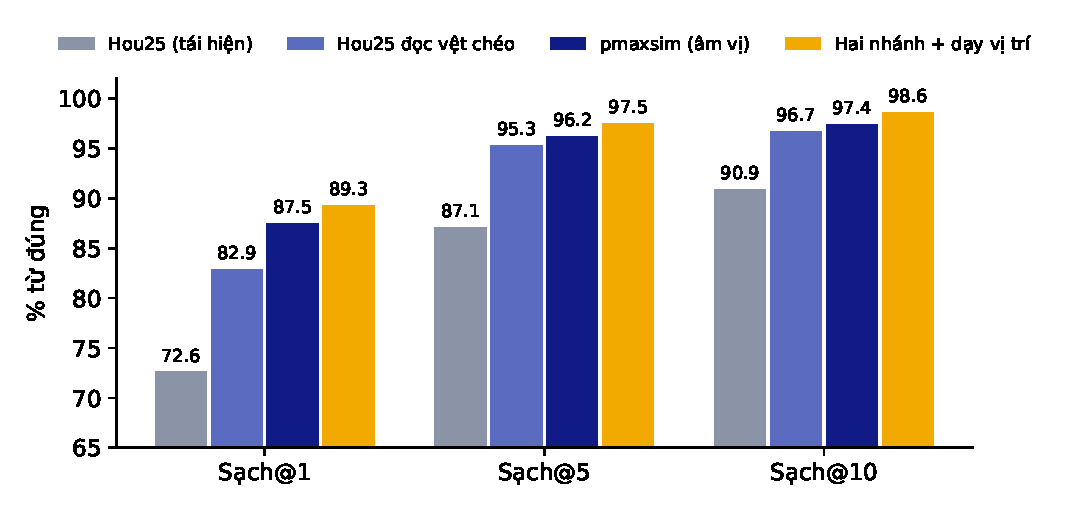
\includegraphics[width=\linewidth,height=3.1cm,keepaspectratio]{imgs/sach_k.pdf}
\par\raggedright
{\tiny Recall@1 / @5 / @10 của 4 scorer. @$K$ = \% từ đúng nằm trong $K$ từ điểm cao nhất (lọc).\par}
\column{0.50\textwidth}
\renewcommand{\arraystretch}{1.05}\scriptsize\setlength{\tabcolsep}{3pt}
\begin{tabular}{L{2.6cm}cc}
\toprule
& top-50 & \textbf{hạng 1} \\
\midrule
\textbf{Hou25} & 95.4 & \bad{72.6} \\
\textbf{âm vị, khớp tự do} & 98.4 & \good{87.5} \\
\midrule
cách nhau & 3.0 & \textbf{14.9} \\
\bottomrule
\end{tabular}
\par\vspace{0.08cm}
{\scriptsize\textbf{Hou25}: nhóm tái hiện paper Interspeech 2025: máy đọc từ \ra{} so 2 đoạn audio \ra{} CNN \ra{} \textbf{trung bình} (trang 10).\par\vspace{0.03cm}
\textbf{Khớp tự do} (code \texttt{pmaxsim}): scorer âm vị bản đầu; mỗi âm vị tìm chỗ giống nhất (trang 17).\par\vspace{0.03cm}
Hou25: 95.4 $-$ 72.6 = 22.8 điểm bị nhiễu vượt. Âm vị: 10.9.\par\vspace{0.04cm}}
{\tiny\color{RiskRed}\textbf{Chưa đo:} Recall@1 cao hơn có chắc làm B-WER thấp hơn không.\par}
\end{columns}
\src{test-other, list N2000, 2939 câu, 5248 lượt từ hiếm; REPORT-1115 mục 3; SMALL\_R N1.}
\end{frame}

% ==================================================================
\section{Vì sao vị trí}
\begin{frame}{Phần 1. Hou25 thua 15 điểm vì đâu?}
\insight{Hou25 thua vì \nb{chấm cao từ nhiễu}, không phải vì chấm thấp từ đúng. Câu càng dài càng nặng.}
\begin{columns}[T]
\column{0.55\textwidth}
\centering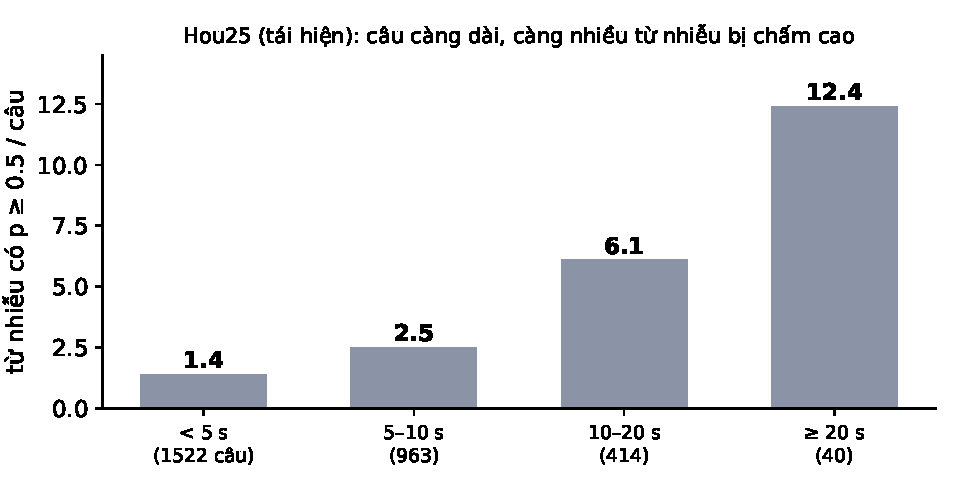
\includegraphics[width=\linewidth]{imgs/bao_nham_hou25.pdf}
\column{0.43\textwidth}
\vspace{0.3cm}
{\small Xét mọi lần từ đúng bị vượt:\par\vspace{0.15cm}
\textbf{\large 96\%} người vượt là từ \textbf{khác hẳn}, không phải từ nghe giống.\par\vspace{0.12cm}
\textbf{\large 76\%} không giống âm nào trong câu.\par\vspace{0.12cm}
\textbf{\large 1.4 \ra{} 12.4} từ nhiễu điểm cao mỗi câu, từ câu ngắn đến câu $\geq$ 20 s.\par}
\end{columns}
\src{test-other N2000; Hou25 nhóm tái hiện (Recall@1 72.6); SMALL\_R N2--N4. Từ nhiễu điểm cao = $p \geq 0.5$.}
\end{frame}

\begin{frame}{Hou25 chấm một từ thế nào}
\insight{Điểm Hou25 = \nb{trung bình điểm của từng ô} trong bảng giống nhau. Mỗi ô chỉ nhìn \nb{9$\times$9 ô quanh nó} (0.18 s) \ra{} không ô nào biết các mảnh sáng có nối nhau không.}
\centering
\begin{tikzpicture}[font=\tiny,>={Stealth},
  b/.style={draw=Primary,fill=SoftBlue,rounded corners=2pt,align=center,inner sep=2pt,minimum height=0.6cm},
  k/.style={draw=Accent,fill=Accent!15,rounded corners=2pt,align=center,inner sep=2pt,minimum height=0.6cm,thick}]
\node[b,text width=1.2cm] (w) at (0,0.4) {từ \texttt{pileser}};
\node[b,text width=1.3cm] (tts) at (1.6,0.4) {máy đọc (TTS)};
\node[b,text width=1.2cm] (a) at (0.8,-0.4) {audio câu};
\node[b,text width=2.4cm] (enc) at (4.0,0) {encoder Whisper đóng băng, 20 ms/khung \ra{} chiếu 368 số};
\node[b,text width=1.5cm] (xa) at (6.45,0) {cross-attention hai chiều};
\node[b,text width=2.0cm] (S) at (8.55,0) {4 bảng cos: hàng = khung câu ($T_s$), cột = khung từ ($T_b$)};
\node[b,text width=1.5cm] (cnn) at (10.65,0) {CNN 4 lớp 3$\times$3: mỗi ô 256 số};
\node[k,text width=1.1cm] (mean) at (12.35,0) {\textbf{trung bình mọi ô}};
\node[b,text width=0.9cm] (o) at (13.75,0) {Linear \ra{} điểm};
\draw[->] (w)--(tts); \draw[->] (tts.east)--(enc.west|-tts.east); \draw[->] (a.east)--(enc.west|-a.east);
\draw[->] (enc)--(xa); \draw[->] (xa)--(S); \draw[->] (S)--(cnn); \draw[->] (cnn)--(mean); \draw[->] (mean)--(o);
\end{tikzpicture}
\vspace{0.12cm}

\begin{columns}[T]
\column{0.52\textwidth}
\nbox{\textbf{Công thức.} $h_{ij}$ = 256 số CNN ra ở ô $(i,j)$; Linear cuối: $w\cdot x + b$.\\[2pt]
\centerline{$\text{điểm} = w\cdot\Big(\frac{1}{T_sT_b}\sum_{i,j} h_{ij}\Big) + b = \frac{1}{T_sT_b}\sum_{i,j} c_{ij} + b$}
với $c_{ij} = w\cdot h_{ij}$ = \textbf{điểm của ô} $(i,j)$. Điểm cả từ = trung bình $c_{ij}$.}
\column{0.45\textwidth}
\nbox[block body alerted]{\textbf{Mỗi ô nhìn bao xa?} 4 lớp tích chập 3$\times$3 \ra{} $c_{ij}$ chỉ phụ thuộc 9$\times$9 ô quanh nó = 0.18 s.\\[2pt]
\ra{} Mảnh sáng ở giây 1 và mảnh ở giây 7 được cộng \textbf{như nhau}, đúng hay sai thứ tự.}
\end{columns}
\src{scorer/models.py, class Hou25 (pool=mean). Cross-attention có nhìn cả câu, nhưng bước gộp cuối vẫn là trung bình từng ô. Paper không có code, nhóm tự cài.}
\end{frame}

\begin{frame}{Trung bình bỏ mất thứ tự: ví dụ số}
\insight{Trung bình chỉ thấy \nb{tổng các ô}: 4 ô sáng rải rác (\nb{0.23}) thắng 3 ô nối chéo (\nb{0.20}). Vệt chéo cộng \nb{dọc đường chéo}: đúng 2.7, nhiễu 1.1.}
\begin{columns}[T]
\column{0.30\textwidth}
\centering
\begin{tikzpicture}[font=\scriptsize]
\def\cs{0.25}
\foreach \gx/\ttl in {0/{ĐÚNG},1.3/{NHIỄU}}{
  \node[font=\scriptsize\bfseries] at (\gx+1.5*\cs,0.2) {\ttl};
  \foreach \rr in {0,...,7}{\foreach \cc in {0,1,2}{\draw[gray!45] (\gx+\cc*\cs,-\rr*\cs) rectangle ++(\cs,-\cs);}}
}
\foreach \rr/\cc in {3/0,4/1,5/2}{\fill[GoodGreen!60] (\cc*\cs,-\rr*\cs) rectangle ++(\cs,-\cs);}
\draw[GoodGreen!70!black,very thick,dashed] (0,-3*\cs) -- (3*\cs,-6*\cs);
\foreach \rr/\cc in {1/2,2/0,5/0,7/1}{\fill[RiskRed!50] (1.3+\cc*\cs,-\rr*\cs) rectangle ++(\cs,-\cs);}
\foreach \rr in {0,...,7}{\node[font=\tiny,anchor=east] at (-0.02,-\rr*\cs-0.5*\cs) {\rr};}
\end{tikzpicture}
\par\raggedright
{\tiny 8 hàng = khung câu, 3 cột = khung từ. Ô màu: $c$ = 0.9; ô trắng: 0.1.\par}
\column{0.68\textwidth}
\renewcommand{\arraystretch}{1.1}\scriptsize\setlength{\tabcolsep}{3pt}
\begin{tabular}{L{3.2cm}L{2.4cm}L{2.4cm}}
\toprule
& từ đúng & từ nhiễu \\
\midrule
\textbf{Trung bình} 24 ô & (3$\times$.9 + 21$\times$.1)/24 = \textbf{0.20} & (4$\times$.9 + 20$\times$.1)/24 = \bad{0.23} \\
\textbf{Vệt chéo}: $\max_{t_0}\sum_j c_{t_0+j,\,j}$ & $t_0$=3: .9+.9+.9 = \good{2.7} & $t_0$=2: .9+.1+.1 = 1.1 \\
\bottomrule
\end{tabular}
\par\vspace{0.1cm}
{\scriptsize\textbf{Chứng minh:} trung bình = (tổng mọi ô)/24. Đổi chỗ các ô, tổng không đổi \ra{} điểm không đổi. Vậy ``3 ô nối chéo'' và ``3 ô rải rác'' \textbf{luôn bằng điểm}: điểm không chứa thứ tự. (Hou25 thật: đổi chỗ được các mảnh cách nhau $>$ 9 ô.)\par\vspace{0.05cm}
\textbf{Câu dài} \ra{} nhiều hàng \ra{} nhiều ô sáng ngẫu nhiên để cộng \ra{} nhiễu điểm cao tăng theo độ dài (trang 9: 1.4 \ra{} 12.4).\par\vspace{0.05cm}
\textbf{Vệt chéo} (ý của Hoàng): chỉ cộng các ô trên một đường chéo, lấy đường tốt nhất; đường đó cho luôn \textbf{chỗ} của từ: hàng $t_0$ tới $t_0+T_b$.\par}
\end{columns}
\src{Ví dụ đồ chơi. Code: models.py, Hou25 pool=mean và pool=diag (diag\_sum). Đường chéo dốc 1: từ máy đọc và từ trong câu phải cùng tốc độ.}
\end{frame}

\begin{frame}{Đo thật: chỉ đổi cách gộp, train lại Hou25}
\insight{Cùng Hou25, cùng lượt train, chỉ đổi bước gộp: vệt chéo \nb{73.3 \ra{} 82.9}. ``Chỗ sáng nhất'' (không đòi thứ tự) chỉ \nb{73.8} \ra{} cái giúp là \nb{thứ tự}.}
\renewcommand{\arraystretch}{1.12}\scriptsize\setlength{\tabcolsep}{3pt}
\begin{tabular}{L{2.4cm}L{4.4cm}ccc}
\toprule
Cách gộp bảng & Làm gì & Recall@1 & nhiễu/câu, câu $\geq$20 s & \% tâm trúng \\
\midrule
Trung bình (Hou25) & trung bình mọi ô (trang 10) & 73.3 & 6.1 & 79\% \\
Chỗ sáng nhất & giữ $T_b$ hàng sáng nhất, \textbf{không cần liền nhau} & 73.8 & 8.0 & 4\% \\
\rowcolor{Accent!15}\textbf{Vệt chéo} (Hoàng) & cộng dọc đường chéo tốt nhất & \good{82.9} & \good{1.9} & \good{99\%} \\
\bottomrule
\end{tabular}
\par\vspace{0.12cm}
{\scriptsize
\textbullet\ \textbf{Recall@1}: \% trong 5248 lượt từ hiếm có từ đúng đứng đầu (trang 6). +9.5 [+7.9; +11.2] \ra{} khác biệt thật.\par
\textbullet\ \textbf{Nhiễu/câu}: số từ nhiễu có $p \geq 0.5$ trung bình mỗi câu dài $\geq$ 20 s (40 câu). Giảm 3 lần: hết ``cộng dồn ô sáng''.\par
\textbullet\ \textbf{\% tâm trúng}: tâm đoạn scorer chỉ ra nằm trong đoạn MFA $\pm$0.1 s. Chỗ sáng nhất 4\%: các hàng sáng nhất \textbf{rải khắp câu}, tâm rơi vào chỗ không có gì.\par
\textbullet\ Chỉ đổi lúc chấm, không train lại \ra{} tệ đi (CNN đã học theo kiểu trung bình).\par}
\src{3 bản Hou25 train cùng lượt (2 epoch), chỉ khác cách gộp; test-other N2000; REPORT-1115 mục 5; A1\_REPORT mục 3.1. Bản Hou25 72.6 ở trang khác là lượt train trước.}
\end{frame}

\begin{frame}{Quyết định D1: sửa Hou25 rồi vẫn thua scorer âm vị}
\insight{Vệt chéo kéo Hou25 từ 72.6 lên \nb{82.9}, nhưng vẫn \nb{dưới} scorer âm vị (85.7). Luật đặt trước: không vượt thì bỏ Hou25 làm nền \ra{} \nb{xây tiếp trên âm vị}.}
\centering
\begin{tikzpicture}[font=\scriptsize,>={Stealth},x=0.62cm]
\draw[->,thick,TextGray] (70,0) -- (90.5,0) node[right] {Recall@1};
\foreach \v in {70,75,80,85,90}{\draw[TextGray] (\v,0.08) -- (\v,-0.08) node[below] {\v};}
\fill[RiskRed] (72.6,0) circle (3.5pt) node[above=4pt,text=RiskRed,align=center] {\textbf{Hou25}\\72.6};
\fill[Accent] (82.9,0) circle (3.5pt) node[above=4pt,align=center] {\textbf{Hou25 vệt chéo}\\82.9};
\draw[->,very thick,Accent] (73.3,0.2) -- node[above] {+ vệt chéo, train lại} (82.3,0.2);
\draw[dashed,thick,Primary] (85.7,-0.3) -- (85.7,0.9) node[right,text=Primary,align=left] {\textbf{luật 85.7}\\= scorer âm vị};
\fill[GoodGreen] (87.5,0) circle (3.5pt) node[below=8pt,text=GoodGreen] {âm vị train lại 87.5};
\end{tikzpicture}
\vspace{0.05cm}

\begin{columns}[T]
\column{0.48\textwidth}
\nbox{\textbf{Âm vị còn hơn:} từ nghe giống 64.7 so với 51.4; nhanh hơn $\sim$200 lần.}
\column{0.48\textwidth}
\nbox[block body alerted]{\textbf{Mang sang:} \hi{thứ tự} \ra{} nhánh khớp đúng thứ tự; \hi{vị trí} \ra{} lọc từ, nhắc Whisper đúng lúc.}
\end{columns}
\src{85.7 = scorer âm vị lúc viết luật; 87.5 = bản train lại sau đó (số ở trang Đo lại ở hạng 1). Hou25 vệt chéo giữ làm đối thủ mạnh. Vệt chéo: ý của Hoàng.}
\end{frame}

% ==================================================================
\section{Scorer}
\begin{frame}{Scorer 1. Scorer đề xuất từ đâu ra}
\insight{Scorer đề xuất = \nb{scorer âm vị} (nền tốt nhất, D1) + \nb{bài học vệt chéo} của phần 1 (đọc đúng thứ tự), gộp trong \nb{một model hai nhánh}.}
\begin{tikzpicture}[font=\scriptsize,>={Stealth},
  s/.style={draw=Primary,fill=SoftBlue,rounded corners=3pt,align=left,inner sep=4pt,text width=2.85cm,minimum height=2.5cm,anchor=north},
  f/.style={draw=Accent,fill=Accent!15,rounded corners=3pt,align=left,inner sep=4pt,text width=2.85cm,minimum height=2.5cm,anchor=north,thick}]
\node[s] (a) at (0,0) {\textbf{1. Phần 1}\\[2pt]Hou25 lấy trung bình \ra{} nhiễu thắng. Bắt đọc theo vệt chéo: \textbf{+9.5}.\\[2pt]\hi{Thứ tự loại được nhiễu.}};
\node[s] (b) at (3.55,0) {\textbf{2. Nền âm vị}\\[2pt]Khớp tự do: mỗi âm vị tìm chỗ giống nhất. \textbf{87.5}, nhưng \textbf{không đòi thứ tự}.};
\node[s] (c) at (7.1,0) {\textbf{3. Thêm thứ tự}\\[2pt]Khớp đúng thứ tự trên âm vị: \textbf{ít nhiễu hơn}, biên chuẩn hơn, nhưng sót nhiều hơn (85.8).};
\node[f] (d) at (10.65,0) {\textbf{4. Gộp + dạy vị trí}\\[2pt]Cộng hai cách: \textbf{+2.6} (hai model cùng kiểu chỉ +1.1) \ra{} bù nhau thật \ra{} \textbf{một model hai nhánh}, dạy vị trí: \good{89.3}.};
\foreach \u/\v in {a/b,b/c,c/d}{\draw[->,very thick,Primary] (\u.east) -- (\v.west);}
\end{tikzpicture}
\vspace{0.25cm}

{\small Tổng quan: trang 15. Từng bước (bảng $M$, tự do, thứ tự, ra $p$, train): trang 16--21. Số đo: trang 22--27.\par}
\src{REPORT-1115 mục 5, 6, 6b, 7c. Tên trong code: khớp tự do = pmaxsim, đúng thứ tự = pmono, đề xuất = pdual2\_dl (scorer/models.py, DualSim).}
\end{frame}

\begin{frame}{Scorer 2. Tổng quan: chấm từ \texttt{pileser} thế nào}
\insight{Lập \nb{bảng giống nhau: âm vị $\times$ thời gian}, rồi đọc bằng \nb{hai nhánh}: nhánh tự do để \nb{không sót}, nhánh đúng thứ tự để \nb{không nhận nhầm} và \nb{ra luôn vị trí}.}
\centering
\begin{tikzpicture}[font=\scriptsize,>={Stealth},
  b/.style={draw=Primary,fill=SoftBlue,rounded corners=2pt,align=center,inner sep=3pt},
  a/.style={draw=Accent,fill=Accent!15,rounded corners=2pt,align=left,inner sep=3pt,thick,text width=3.7cm},
  o/.style={draw=GoodGreen,fill=GoodGreen!12,rounded corners=2pt,align=center,inner sep=3pt}]
% đầu vào
\node[b,text width=2.6cm] (au) at (0,0.55) {\textbf{audio câu}\\encoder Whisper (đóng băng)\\mỗi 20 ms một vector};
\node[b,text width=2.6cm] (wd) at (0,-1.45) {\textbf{từ} \texttt{pileser}\\P AY L IY Z ER\\mỗi âm vị một vector\\{\tiny (tính sẵn cho cả kho)}};
% bảng
\def\cs{0.27}
\def\ox{2.25}\def\oy{0.45}
\foreach \rr in {0,...,5}{\foreach \cc in {0,...,11}{\draw[gray!45] (\ox+\cc*\cs,\oy-\rr*\cs) rectangle ++(\cs,-\cs);}}
\foreach \rr/\cc in {0/2,1/3,2/4,3/5,4/7,5/8}{\fill[GoodGreen!65] (\ox+\cc*\cs,\oy-\rr*\cs) rectangle ++(\cs,-\cs);}
\foreach \rr/\cc in {1/10,3/0}{\fill[Accent!70] (\ox+\cc*\cs,\oy-\rr*\cs) rectangle ++(\cs,-\cs);}
\draw[GoodGreen!60!black,very thick] (\ox+2.5*\cs,\oy-0.5*\cs) -- (\ox+3.5*\cs,\oy-1.5*\cs) -- (\ox+4.5*\cs,\oy-2.5*\cs) -- (\ox+5.5*\cs,\oy-3.5*\cs) -- (\ox+7.5*\cs,\oy-4.5*\cs) -- (\ox+8.5*\cs,\oy-5.5*\cs);
\foreach \ph [count=\i from 0] in {P,AY,L,IY,Z,ER}{\node[font=\tiny,anchor=east] at (\ox-0.02,\oy-\i*\cs-0.5*\cs) {\ph};}
\node[font=\tiny,anchor=south] at (\ox+6*\cs,\oy+0.02) {thời gian câu \ra};
\node[font=\tiny,align=center,anchor=north] at (\ox+6*\cs,\oy-6*\cs-0.05) {ô = độ giống (âm vị, khung 20 ms)\\\textcolor{GoodGreen!60!black}{xanh}: đường đúng thứ tự;\ \textcolor{Accent}{vàng}: ô sáng lẻ};
\draw[->,thick] (au.east) -- (\ox-0.35,\oy-1.5*\cs);
\draw[->,thick] (wd.east) -- (\ox-0.35,\oy-4.5*\cs);
% hai nhánh
\node[a] (n1) at (8.55,0.75) {\textbf{Nhánh tự do}: mỗi âm vị lấy ô sáng nhất trong hàng, ở đâu cũng được \ra{} \textbf{ít sót}};
\node[a] (n2) at (8.55,-1.05) {\textbf{Nhánh đúng thứ tự}: đường đi từ trên xuống, sang phải; âm vị sau cách âm vị trước $\leq$ 0.3 s \ra{} \textbf{ít nhiễu}, cho [đầu, cuối]};
\node[o,text width=1.75cm] (out) at (12.15,-0.1) {cộng điểm\\\ra{} (từ, $p$, đầu, cuối)};
\draw[->,thick] (\ox+12*\cs+0.05,\oy-1.5*\cs) -- (n1.west);
\draw[->,thick] (\ox+12*\cs+0.05,\oy-3.5*\cs) -- (n2.west);
\draw[->,thick] (n1.east) -- (out.west); \draw[->,thick] (n2.east) -- (out.west);
\end{tikzpicture}
\vspace{0.1cm}

\raggedright
{\scriptsize\textbullet\ Khác vệt chéo của Hou25: đường đi cho phép \textbf{nói nhanh, nói chậm}, không bắt mỗi bước đúng một khung.\par
\textbullet\ Mỗi nhánh có \textbf{bảng riêng} (dùng chung một bảng chỉ 88.3, so với 89.3).\par
\textbullet\ \textbf{Dạy vị trí} lúc train: từ đúng chỉ được khớp trong đoạn nó thật sự được nói (căn chỉnh MFA $\pm$0.1 s).\par}
\src{scorer/models.py: DualSim(two=True). 5.4 M tham số, chấm 4--7 ms/câu. Train 6 epoch trên train-clean-100, chọn checkpoint trên dev-other.}
\end{frame}

\begin{frame}{Scorer 3. Bước 1: từ \ra{} âm vị, audio \ra{} khung, rồi lập bảng $M$}
\insight{Từ thành \nb{dãy âm vị}, mỗi 20 ms audio thành \nb{một khung}. $M$[âm vị, khung] = \nb{độ giống} (cos). Mọi bước sau chỉ là \nb{đọc bảng này}.}
\begin{columns}[T]
\column{0.55\textwidth}
\scriptsize
\textcolor{Primary}{\textbf{1. Từ \ra{} âm vị (G2P).}} \texttt{g2p\_en} tra từ điển phát âm CMUdict; không có thì mạng seq2seq đoán. \texttt{pileser} \ra{} P AY1 L IY0 Z ER0 \ra{} bỏ số trọng âm \ra{} \textbf{P AY L IY Z ER} ($P$ = 6; bộ $\sim$40 âm vị).\par\vspace{0.05cm}
\textcolor{Primary}{\textbf{2. Âm vị \ra{} vector.}} Mỗi âm vị 1 vector 256 số + vector ``vị trí trong từ'' \ra{} 2 lớp Transformer \ra{} $e_1..e_P$. Không phụ thuộc câu \ra{} \textbf{tính sẵn một lần cho kho 209k từ}.\par\vspace{0.05cm}
\textcolor{Primary}{\textbf{3. Audio \ra{} vector.}} Encoder Whisper-large-v3 (đóng băng): 20 ms một vector 1280 số \ra{} chiếu 256 + 1 lớp Transformer \ra{} $s_1..s_T$. Câu 10 s: $T$ = 500.\par\vspace{0.05cm}
\textcolor{Primary}{\textbf{4. Bảng.}} Chuẩn hoá độ dài 1 \ra{} $M[p,t] = e_p \cdot s_t$ = cos, từ $-1$ tới 1.\par
\column{0.43\textwidth}
\centering
\begin{tikzpicture}[font=\tiny]
\def\cs{0.22}
\foreach \rr in {0,...,5}{\foreach \cc in {0,...,15}{\draw[gray!40] (\cc*\cs,-\rr*\cs) rectangle ++(\cs,-\cs);}}
\foreach \rr/\cc in {0/3,1/4,2/6,3/7,4/9,5/10}{\fill[Primary!70] (\cc*\cs,-\rr*\cs) rectangle ++(\cs,-\cs);}
\foreach \rr/\cc in {1/13,3/1,0/14}{\fill[Primary!35] (\cc*\cs,-\rr*\cs) rectangle ++(\cs,-\cs);}
\foreach \ph [count=\i from 0] in {P,AY,L,IY,Z,ER}{\node[anchor=east] at (-0.02,-\i*\cs-0.5*\cs) {\ph};}
\node[anchor=south] at (8*\cs,0.02) {khung câu (20 ms) \ra};
\node[anchor=north] at (8*\cs,-6*\cs-0.03) {bảng $M$ của \texttt{pileser}: ô đậm = giống};
\end{tikzpicture}
\par\vspace{0.1cm}\raggedright
{\scriptsize\textbf{Câu 10 s, list 2000 từ:} mỗi từ một bảng $\sim$6$\times$500 ô; cả list = \textbf{1 phép nhân ma trận}, 4--7 ms/câu (Hou25 $\sim$1200 ms).\par\vspace{0.05cm}
Đề xuất có \textbf{hai bộ chiếu riêng} \ra{} hai bảng $M^{\text{tự do}}$, $M^{\text{thứ tự}}$ (trang 20).\par}
\end{columns}
\src{scorer/data/g2p.py; scorer/models.py: PhoneEnc (256 chiều, 2 lớp, 4 head), DualSim. Hou25 chậm vì phải đọc TTS từng từ rồi qua encoder.}
\end{frame}

\begin{frame}{Scorer 4. Khớp tự do: mỗi âm vị lấy ô sáng nhất}
\insight{Điểm tự do = trung bình \nb{ô sáng nhất mỗi hàng}, không hỏi các ô đó \nb{có theo thứ tự không} \ra{} nhiễu rải rác vẫn được \nb{0.75}, gần từ đúng \nb{0.85}.}
\begin{columns}[T]
\column{0.46\textwidth}
\nbox{\centering$\text{tự do} = \dfrac{1}{P}\sum_{p=1}^{P}\ \max_{t}\ M[p,t]$\\[2pt]
\raggedright\scriptsize mỗi âm vị $p$ (hàng): tìm khung $t$ giống nhất, ở đâu cũng được; rồi trung bình $P$ số đó.}
\vspace{0.1cm}
{\scriptsize\textbf{Ví dụ} 4 âm vị $\times$ 8 khung (viền vàng = ô được chọn):\par
\textbullet\ Đúng: khung 2, 3, 4, 6 \ra{} (.9+.8+.9+.8)/4 = \textbf{0.85}.\par
\textbullet\ Nhiễu: khung \textbf{5, 0, 7, 1} (lộn xộn) \ra{} (.8+.7+.8+.7)/4 = \bad{0.75}.\par\vspace{0.06cm}
\textbf{Vị trí:} tâm = trung vị các khung được chọn; rộng 4 khung mỗi âm vị ($\approx$80 ms).\par
Đúng: trung vị(2,3,4,6) = 3.5. Nhiễu: trung vị(0,1,5,7) = 3, \textbf{giữa hai cụm}, chỗ không có gì.\par}
\column{0.52\textwidth}
\centering
\begin{tikzpicture}
\fill[Primary!14] (0.00,0.00) rectangle ++(0.29,-0.29);
\draw[gray!40] (0.00,0.00) rectangle ++(0.29,-0.29);
\node[font=\tiny,text=black] at (0.14,-0.14) {.2};
\fill[Primary!7] (0.29,0.00) rectangle ++(0.29,-0.29);
\draw[gray!40] (0.29,0.00) rectangle ++(0.29,-0.29);
\node[font=\tiny,text=black] at (0.43,-0.14) {.1};
\fill[Primary!63] (0.58,0.00) rectangle ++(0.29,-0.29);
\draw[gray!40] (0.58,0.00) rectangle ++(0.29,-0.29);
\node[font=\tiny,text=white] at (0.72,-0.14) {.9};
\fill[Primary!14] (0.87,0.00) rectangle ++(0.29,-0.29);
\draw[gray!40] (0.87,0.00) rectangle ++(0.29,-0.29);
\node[font=\tiny,text=black] at (1.01,-0.14) {.2};
\fill[Primary!7] (1.16,0.00) rectangle ++(0.29,-0.29);
\draw[gray!40] (1.16,0.00) rectangle ++(0.29,-0.29);
\node[font=\tiny,text=black] at (1.30,-0.14) {.1};
\fill[Primary!14] (1.45,0.00) rectangle ++(0.29,-0.29);
\draw[gray!40] (1.45,0.00) rectangle ++(0.29,-0.29);
\node[font=\tiny,text=black] at (1.59,-0.14) {.2};
\fill[Primary!7] (1.74,0.00) rectangle ++(0.29,-0.29);
\draw[gray!40] (1.74,0.00) rectangle ++(0.29,-0.29);
\node[font=\tiny,text=black] at (1.88,-0.14) {.1};
\fill[Primary!14] (2.03,0.00) rectangle ++(0.29,-0.29);
\draw[gray!40] (2.03,0.00) rectangle ++(0.29,-0.29);
\node[font=\tiny,text=black] at (2.17,-0.14) {.2};
\fill[Primary!7] (0.00,-0.29) rectangle ++(0.29,-0.29);
\draw[gray!40] (0.00,-0.29) rectangle ++(0.29,-0.29);
\node[font=\tiny,text=black] at (0.14,-0.43) {.1};
\fill[Primary!14] (0.29,-0.29) rectangle ++(0.29,-0.29);
\draw[gray!40] (0.29,-0.29) rectangle ++(0.29,-0.29);
\node[font=\tiny,text=black] at (0.43,-0.43) {.2};
\fill[Primary!21] (0.58,-0.29) rectangle ++(0.29,-0.29);
\draw[gray!40] (0.58,-0.29) rectangle ++(0.29,-0.29);
\node[font=\tiny,text=black] at (0.72,-0.43) {.3};
\fill[Primary!56] (0.87,-0.29) rectangle ++(0.29,-0.29);
\draw[gray!40] (0.87,-0.29) rectangle ++(0.29,-0.29);
\node[font=\tiny,text=white] at (1.01,-0.43) {.8};
\fill[Primary!14] (1.16,-0.29) rectangle ++(0.29,-0.29);
\draw[gray!40] (1.16,-0.29) rectangle ++(0.29,-0.29);
\node[font=\tiny,text=black] at (1.30,-0.43) {.2};
\fill[Primary!7] (1.45,-0.29) rectangle ++(0.29,-0.29);
\draw[gray!40] (1.45,-0.29) rectangle ++(0.29,-0.29);
\node[font=\tiny,text=black] at (1.59,-0.43) {.1};
\fill[Primary!14] (1.74,-0.29) rectangle ++(0.29,-0.29);
\draw[gray!40] (1.74,-0.29) rectangle ++(0.29,-0.29);
\node[font=\tiny,text=black] at (1.88,-0.43) {.2};
\fill[Primary!7] (2.03,-0.29) rectangle ++(0.29,-0.29);
\draw[gray!40] (2.03,-0.29) rectangle ++(0.29,-0.29);
\node[font=\tiny,text=black] at (2.17,-0.43) {.1};
\fill[Primary!14] (0.00,-0.58) rectangle ++(0.29,-0.29);
\draw[gray!40] (0.00,-0.58) rectangle ++(0.29,-0.29);
\node[font=\tiny,text=black] at (0.14,-0.72) {.2};
\fill[Primary!7] (0.29,-0.58) rectangle ++(0.29,-0.29);
\draw[gray!40] (0.29,-0.58) rectangle ++(0.29,-0.29);
\node[font=\tiny,text=black] at (0.43,-0.72) {.1};
\fill[Primary!14] (0.58,-0.58) rectangle ++(0.29,-0.29);
\draw[gray!40] (0.58,-0.58) rectangle ++(0.29,-0.29);
\node[font=\tiny,text=black] at (0.72,-0.72) {.2};
\fill[Primary!14] (0.87,-0.58) rectangle ++(0.29,-0.29);
\draw[gray!40] (0.87,-0.58) rectangle ++(0.29,-0.29);
\node[font=\tiny,text=black] at (1.01,-0.72) {.2};
\fill[Primary!63] (1.16,-0.58) rectangle ++(0.29,-0.29);
\draw[gray!40] (1.16,-0.58) rectangle ++(0.29,-0.29);
\node[font=\tiny,text=white] at (1.30,-0.72) {.9};
\fill[Primary!21] (1.45,-0.58) rectangle ++(0.29,-0.29);
\draw[gray!40] (1.45,-0.58) rectangle ++(0.29,-0.29);
\node[font=\tiny,text=black] at (1.59,-0.72) {.3};
\fill[Primary!7] (1.74,-0.58) rectangle ++(0.29,-0.29);
\draw[gray!40] (1.74,-0.58) rectangle ++(0.29,-0.29);
\node[font=\tiny,text=black] at (1.88,-0.72) {.1};
\fill[Primary!14] (2.03,-0.58) rectangle ++(0.29,-0.29);
\draw[gray!40] (2.03,-0.58) rectangle ++(0.29,-0.29);
\node[font=\tiny,text=black] at (2.17,-0.72) {.2};
\fill[Primary!7] (0.00,-0.87) rectangle ++(0.29,-0.29);
\draw[gray!40] (0.00,-0.87) rectangle ++(0.29,-0.29);
\node[font=\tiny,text=black] at (0.14,-1.01) {.1};
\fill[Primary!14] (0.29,-0.87) rectangle ++(0.29,-0.29);
\draw[gray!40] (0.29,-0.87) rectangle ++(0.29,-0.29);
\node[font=\tiny,text=black] at (0.43,-1.01) {.2};
\fill[Primary!7] (0.58,-0.87) rectangle ++(0.29,-0.29);
\draw[gray!40] (0.58,-0.87) rectangle ++(0.29,-0.29);
\node[font=\tiny,text=black] at (0.72,-1.01) {.1};
\fill[Primary!14] (0.87,-0.87) rectangle ++(0.29,-0.29);
\draw[gray!40] (0.87,-0.87) rectangle ++(0.29,-0.29);
\node[font=\tiny,text=black] at (1.01,-1.01) {.2};
\fill[Primary!14] (1.16,-0.87) rectangle ++(0.29,-0.29);
\draw[gray!40] (1.16,-0.87) rectangle ++(0.29,-0.29);
\node[font=\tiny,text=black] at (1.30,-1.01) {.2};
\fill[Primary!14] (1.45,-0.87) rectangle ++(0.29,-0.29);
\draw[gray!40] (1.45,-0.87) rectangle ++(0.29,-0.29);
\node[font=\tiny,text=black] at (1.59,-1.01) {.2};
\fill[Primary!56] (1.74,-0.87) rectangle ++(0.29,-0.29);
\draw[gray!40] (1.74,-0.87) rectangle ++(0.29,-0.29);
\node[font=\tiny,text=white] at (1.88,-1.01) {.8};
\fill[Primary!7] (2.03,-0.87) rectangle ++(0.29,-0.29);
\draw[gray!40] (2.03,-0.87) rectangle ++(0.29,-0.29);
\node[font=\tiny,text=black] at (2.17,-1.01) {.1};
\draw[Accent,line width=1.4pt] (0.58,0.00) rectangle ++(0.29,-0.29);
\draw[Accent,line width=1.4pt] (0.87,-0.29) rectangle ++(0.29,-0.29);
\draw[Accent,line width=1.4pt] (1.16,-0.58) rectangle ++(0.29,-0.29);
\draw[Accent,line width=1.4pt] (1.74,-0.87) rectangle ++(0.29,-0.29);
\node[font=\tiny,text=TextGray] at (0.14,0.15) {0};
\node[font=\tiny,text=TextGray] at (0.43,0.15) {1};
\node[font=\tiny,text=TextGray] at (0.72,0.15) {2};
\node[font=\tiny,text=TextGray] at (1.01,0.15) {3};
\node[font=\tiny,text=TextGray] at (1.30,0.15) {4};
\node[font=\tiny,text=TextGray] at (1.59,0.15) {5};
\node[font=\tiny,text=TextGray] at (1.88,0.15) {6};
\node[font=\tiny,text=TextGray] at (2.17,0.15) {7};
\node[font=\scriptsize\bfseries,anchor=south] at (1.16,0.28) {từ đúng: khung 2, 3, 4, 6};
\begin{scope}[yshift=-2.05cm]
\fill[Primary!14] (0.00,0.00) rectangle ++(0.29,-0.29);
\draw[gray!40] (0.00,0.00) rectangle ++(0.29,-0.29);
\node[font=\tiny,text=black] at (0.14,-0.14) {.2};
\fill[Primary!7] (0.29,0.00) rectangle ++(0.29,-0.29);
\draw[gray!40] (0.29,0.00) rectangle ++(0.29,-0.29);
\node[font=\tiny,text=black] at (0.43,-0.14) {.1};
\fill[Primary!14] (0.58,0.00) rectangle ++(0.29,-0.29);
\draw[gray!40] (0.58,0.00) rectangle ++(0.29,-0.29);
\node[font=\tiny,text=black] at (0.72,-0.14) {.2};
\fill[Primary!7] (0.87,0.00) rectangle ++(0.29,-0.29);
\draw[gray!40] (0.87,0.00) rectangle ++(0.29,-0.29);
\node[font=\tiny,text=black] at (1.01,-0.14) {.1};
\fill[Primary!14] (1.16,0.00) rectangle ++(0.29,-0.29);
\draw[gray!40] (1.16,0.00) rectangle ++(0.29,-0.29);
\node[font=\tiny,text=black] at (1.30,-0.14) {.2};
\fill[Primary!56] (1.45,0.00) rectangle ++(0.29,-0.29);
\draw[gray!40] (1.45,0.00) rectangle ++(0.29,-0.29);
\node[font=\tiny,text=white] at (1.59,-0.14) {.8};
\fill[Primary!7] (1.74,0.00) rectangle ++(0.29,-0.29);
\draw[gray!40] (1.74,0.00) rectangle ++(0.29,-0.29);
\node[font=\tiny,text=black] at (1.88,-0.14) {.1};
\fill[Primary!14] (2.03,0.00) rectangle ++(0.29,-0.29);
\draw[gray!40] (2.03,0.00) rectangle ++(0.29,-0.29);
\node[font=\tiny,text=black] at (2.17,-0.14) {.2};
\fill[Primary!49] (0.00,-0.29) rectangle ++(0.29,-0.29);
\draw[gray!40] (0.00,-0.29) rectangle ++(0.29,-0.29);
\node[font=\tiny,text=white] at (0.14,-0.43) {.7};
\fill[Primary!14] (0.29,-0.29) rectangle ++(0.29,-0.29);
\draw[gray!40] (0.29,-0.29) rectangle ++(0.29,-0.29);
\node[font=\tiny,text=black] at (0.43,-0.43) {.2};
\fill[Primary!7] (0.58,-0.29) rectangle ++(0.29,-0.29);
\draw[gray!40] (0.58,-0.29) rectangle ++(0.29,-0.29);
\node[font=\tiny,text=black] at (0.72,-0.43) {.1};
\fill[Primary!14] (0.87,-0.29) rectangle ++(0.29,-0.29);
\draw[gray!40] (0.87,-0.29) rectangle ++(0.29,-0.29);
\node[font=\tiny,text=black] at (1.01,-0.43) {.2};
\fill[Primary!7] (1.16,-0.29) rectangle ++(0.29,-0.29);
\draw[gray!40] (1.16,-0.29) rectangle ++(0.29,-0.29);
\node[font=\tiny,text=black] at (1.30,-0.43) {.1};
\fill[Primary!14] (1.45,-0.29) rectangle ++(0.29,-0.29);
\draw[gray!40] (1.45,-0.29) rectangle ++(0.29,-0.29);
\node[font=\tiny,text=black] at (1.59,-0.43) {.2};
\fill[Primary!14] (1.74,-0.29) rectangle ++(0.29,-0.29);
\draw[gray!40] (1.74,-0.29) rectangle ++(0.29,-0.29);
\node[font=\tiny,text=black] at (1.88,-0.43) {.2};
\fill[Primary!7] (2.03,-0.29) rectangle ++(0.29,-0.29);
\draw[gray!40] (2.03,-0.29) rectangle ++(0.29,-0.29);
\node[font=\tiny,text=black] at (2.17,-0.43) {.1};
\fill[Primary!7] (0.00,-0.58) rectangle ++(0.29,-0.29);
\draw[gray!40] (0.00,-0.58) rectangle ++(0.29,-0.29);
\node[font=\tiny,text=black] at (0.14,-0.72) {.1};
\fill[Primary!14] (0.29,-0.58) rectangle ++(0.29,-0.29);
\draw[gray!40] (0.29,-0.58) rectangle ++(0.29,-0.29);
\node[font=\tiny,text=black] at (0.43,-0.72) {.2};
\fill[Primary!14] (0.58,-0.58) rectangle ++(0.29,-0.29);
\draw[gray!40] (0.58,-0.58) rectangle ++(0.29,-0.29);
\node[font=\tiny,text=black] at (0.72,-0.72) {.2};
\fill[Primary!7] (0.87,-0.58) rectangle ++(0.29,-0.29);
\draw[gray!40] (0.87,-0.58) rectangle ++(0.29,-0.29);
\node[font=\tiny,text=black] at (1.01,-0.72) {.1};
\fill[Primary!14] (1.16,-0.58) rectangle ++(0.29,-0.29);
\draw[gray!40] (1.16,-0.58) rectangle ++(0.29,-0.29);
\node[font=\tiny,text=black] at (1.30,-0.72) {.2};
\fill[Primary!7] (1.45,-0.58) rectangle ++(0.29,-0.29);
\draw[gray!40] (1.45,-0.58) rectangle ++(0.29,-0.29);
\node[font=\tiny,text=black] at (1.59,-0.72) {.1};
\fill[Primary!14] (1.74,-0.58) rectangle ++(0.29,-0.29);
\draw[gray!40] (1.74,-0.58) rectangle ++(0.29,-0.29);
\node[font=\tiny,text=black] at (1.88,-0.72) {.2};
\fill[Primary!56] (2.03,-0.58) rectangle ++(0.29,-0.29);
\draw[gray!40] (2.03,-0.58) rectangle ++(0.29,-0.29);
\node[font=\tiny,text=white] at (2.17,-0.72) {.8};
\fill[Primary!14] (0.00,-0.87) rectangle ++(0.29,-0.29);
\draw[gray!40] (0.00,-0.87) rectangle ++(0.29,-0.29);
\node[font=\tiny,text=black] at (0.14,-1.01) {.2};
\fill[Primary!49] (0.29,-0.87) rectangle ++(0.29,-0.29);
\draw[gray!40] (0.29,-0.87) rectangle ++(0.29,-0.29);
\node[font=\tiny,text=white] at (0.43,-1.01) {.7};
\fill[Primary!7] (0.58,-0.87) rectangle ++(0.29,-0.29);
\draw[gray!40] (0.58,-0.87) rectangle ++(0.29,-0.29);
\node[font=\tiny,text=black] at (0.72,-1.01) {.1};
\fill[Primary!14] (0.87,-0.87) rectangle ++(0.29,-0.29);
\draw[gray!40] (0.87,-0.87) rectangle ++(0.29,-0.29);
\node[font=\tiny,text=black] at (1.01,-1.01) {.2};
\fill[Primary!7] (1.16,-0.87) rectangle ++(0.29,-0.29);
\draw[gray!40] (1.16,-0.87) rectangle ++(0.29,-0.29);
\node[font=\tiny,text=black] at (1.30,-1.01) {.1};
\fill[Primary!14] (1.45,-0.87) rectangle ++(0.29,-0.29);
\draw[gray!40] (1.45,-0.87) rectangle ++(0.29,-0.29);
\node[font=\tiny,text=black] at (1.59,-1.01) {.2};
\fill[Primary!7] (1.74,-0.87) rectangle ++(0.29,-0.29);
\draw[gray!40] (1.74,-0.87) rectangle ++(0.29,-0.29);
\node[font=\tiny,text=black] at (1.88,-1.01) {.1};
\fill[Primary!14] (2.03,-0.87) rectangle ++(0.29,-0.29);
\draw[gray!40] (2.03,-0.87) rectangle ++(0.29,-0.29);
\node[font=\tiny,text=black] at (2.17,-1.01) {.2};
\draw[Accent,line width=1.4pt] (1.45,0.00) rectangle ++(0.29,-0.29);
\draw[Accent,line width=1.4pt] (0.00,-0.29) rectangle ++(0.29,-0.29);
\draw[Accent,line width=1.4pt] (2.03,-0.58) rectangle ++(0.29,-0.29);
\draw[Accent,line width=1.4pt] (0.29,-0.87) rectangle ++(0.29,-0.29);
\node[font=\tiny,text=TextGray] at (0.14,0.15) {0};
\node[font=\tiny,text=TextGray] at (0.43,0.15) {1};
\node[font=\tiny,text=TextGray] at (0.72,0.15) {2};
\node[font=\tiny,text=TextGray] at (1.01,0.15) {3};
\node[font=\tiny,text=TextGray] at (1.30,0.15) {4};
\node[font=\tiny,text=TextGray] at (1.59,0.15) {5};
\node[font=\tiny,text=TextGray] at (1.88,0.15) {6};
\node[font=\tiny,text=TextGray] at (2.17,0.15) {7};
\node[font=\scriptsize\bfseries,anchor=south] at (1.16,0.28) {từ nhiễu: khung 5, 0, 7, 1};
\end{scope}
\end{tikzpicture}
\end{columns}
\src{scorer/models.py: MaxSim. Số thật của khớp tự do (\texttt{pmaxsim}): trang 22. Ví dụ đồ chơi, không phải số đo.}
\end{frame}

\begin{frame}{Scorer 5. Khớp đúng thứ tự: tính bảng $D$ từng bước}
\insight{$D[p,t]$ = điểm \nb{đường tốt nhất} qua âm vị 1..$p$, \nb{kết thúc ở khung $t$}. Từ đúng: hàng cuối đạt 3.4 \ra{} 3.4/4 = \nb{0.85}.}
\begin{columns}[T]
\column{0.42\textwidth}
\nbox{\centering$D[1,t] = M[1,t]$\\[1pt]
$D[p,t] = M[p,t] + \max\limits_{1\le g\le G} D[p-1,\,t-g]$\\[1pt]
$\text{thứ tự} = \max_t D[P,t]\ /\ P$}
\vspace{0.06cm}
{\scriptsize\textbf{Đọc:} âm vị $p$ ở khung $t$ thì âm vị trước phải ở \textbf{trước đó} 1..$G$ khung. Thật: $G$ = 15 khung (0.3 s); ví dụ: $G$ = 2.\par\vspace{0.05cm}
\textbf{Ba ô tính tay} (ô xanh):\par
$D[2,3]$ = .8 + max(.9, .1) = \textbf{1.7}\par
$D[3,4]$ = .9 + max(1.7, .5) = \textbf{2.6}\par
$D[4,6]$ = .8 + max(2.0, 2.6) = \textbf{3.4}\par
{\tiny (hai số trong max = $D$ của hàng trên, 1 và 2 khung trước)\par}}
\column{0.56\textwidth}
\renewcommand{\arraystretch}{1.0}\scriptsize\setlength{\tabcolsep}{3.2pt}
\textbf{Bảng $M$ (từ đúng)}\par
\begin{tabular}{c|cccccccc}
khung & 0&1&2&3&4&5&6&7\\\hline
âm vị 1 & .2&.1&\cellcolor{GoodGreen!35}.9&.2&.1&.2&.1&.2\\
âm vị 2 & .1&.2&.3&\cellcolor{GoodGreen!35}.8&.2&.1&.2&.1\\
âm vị 3 & .2&.1&.2&.2&\cellcolor{GoodGreen!35}.9&.3&.1&.2\\
âm vị 4 & .1&.2&.1&.2&.2&.2&\cellcolor{GoodGreen!35}.8&.1\\
\end{tabular}
\par\vspace{0.08cm}
\textbf{Bảng $D$} ($-$ = chưa đủ khung phía trước, không có đường)\par
\begin{tabular}{c|cccccccc}
khung & 0&1&2&3&4&5&6&7\\\hline
$p$=1 & .2&.1&\cellcolor{GoodGreen!35}.9&.2&.1&.2&.1&.2\\
$p$=2 & $-$&.4&.5&\cellcolor{GoodGreen!35}1.7&1.1&.3&.4&.3\\
$p$=3 & $-$&$-$&.6&.7&\cellcolor{GoodGreen!35}2.6&2.0&1.2&.6\\
$p$=4 & $-$&$-$&$-$&.8&.9&2.8&\cellcolor{GoodGreen!35}\textbf{3.4}&2.1\\
\end{tabular}
\par\vspace{0.05cm}
{\tiny Tự do cũng 0.85: ở từ đúng, các ô sáng nhất \textbf{đã} theo thứ tự.\par}
\end{columns}
\src{scorer/models.py: MonoSim. Cài bằng max\_pool1d cỡ $G$ trượt theo thời gian: mỗi hàng 1 phép.}
\end{frame}

\begin{frame}{Scorer 6. Từ nhiễu bị chặn, và lần ngược ra vị trí}
\insight{Nhiễu có ô sáng nhưng \nb{sai thứ tự} \ra{} chỉ còn \nb{0.20} (tự do: 0.75). Lần ngược đường của từ đúng \ra{} \nb{khung 2--6}.}
\begin{columns}[T]
\column{0.52\textwidth}
\renewcommand{\arraystretch}{0.95}\tiny\setlength{\tabcolsep}{3.2pt}
\textbf{Từ nhiễu: bảng $M$} (ô sáng ở khung 5, 0, 7, 1)\par
\begin{tabular}{c|cccccccc}
khung & 0&1&2&3&4&5&6&7\\\hline
âm vị 1 & .2&.1&.2&.1&.2&\cellcolor{RiskRed!25}.8&.1&.2\\
âm vị 2 & \cellcolor{RiskRed!25}.7&.2&.1&.2&.1&.2&.2&.1\\
âm vị 3 & .1&.2&.2&.1&.2&.1&.2&\cellcolor{RiskRed!25}.8\\
âm vị 4 & .2&\cellcolor{RiskRed!25}.7&.1&.2&.1&.2&.1&.2\\
\end{tabular}
\par\vspace{0.06cm}
\textbf{Bảng $D$}\par
\begin{tabular}{c|cccccccc}
khung & 0&1&2&3&4&5&6&7\\\hline
$p$=1 & .2&.1&.2&.1&.2&\cellcolor{Accent!30}.8&.1&.2\\
$p$=2 & $-$&.4&.3&.4&.3&.4&\cellcolor{Accent!30}1.0&.9\\
$p$=3 & $-$&$-$&.6&.5&.6&.5&.6&\cellcolor{Accent!30}1.8\\
$p$=4 & $-$&$-$&$-$&\textbf{.8}&.7&.8&.7&.8\\
\end{tabular}
\par\vspace{0.04cm}
{\tiny Vàng: đường qua ô sáng tới 1.8 ở khung 7; âm vị 4 phải ở \textbf{sau} khung 7 \ra{} hết chỗ. Tốt nhất: 0.8/4 = 0.20.\par}
\column{0.46\textwidth}
\nbox{\textbf{Lần ngược ra vị trí} (từ đúng, trang 18)\\[2pt]
\scriptsize
Khi tính $D$, nhớ mỗi ô lấy max từ ô nào.\\
$p$=4: max hàng cuối 3.4 ở \textbf{khung 6} = \textbf{cuối từ}\\
$p$=3: 3.4 lấy từ $D[3,4]$ = 2.6 \ra{} khung 4\\
$p$=2: 2.6 lấy từ $D[2,3]$ = 1.7 \ra{} khung 3\\
$p$=1: 1.7 lấy từ $D[1,2]$ = .9 \ra{} \textbf{khung 2 = đầu từ}\\[2pt]
\ra{} từ ở khung \textbf{2--6} = 0.04--0.14 s.}
\vspace{0.08cm}
{\scriptsize\textbf{Vì sao chuẩn hơn tự do?} Tự do lấy trung vị các ô chọn: một âm vị phổ biến (vd.\ ER) khớp chỗ khác sẽ \textbf{kéo tâm lệch}. Thứ tự buộc mọi âm vị nằm \textbf{liền một đoạn} (diễn giải; số đo trang 22--23).\par}
\end{columns}
\src{Ví dụ đồ chơi, $G$ = 2. Code: MonoSim lưu khung bắt đầu của đường qua chỉ số của max\_pool1d.}
\end{frame}

\begin{frame}{Scorer 7. Từ hai điểm ra xác suất $p$}
\insight{$\text{logit} = a\cdot\text{thứ tự} + a_2\cdot\text{tự do} + c$, $p$ = sigmoid(logit). Nhiễu rải rác: chỉ tự do cho \nb{$p$ = 0.92} (lọt ngưỡng 0.5); thêm thứ tự còn \nb{0.38} (bị loại).}
\begin{columns}[T]
\column{0.52\textwidth}
\renewcommand{\arraystretch}{1.1}\scriptsize\setlength{\tabcolsep}{3pt}
\begin{tabular}{L{3.3cm}L{1.6cm}L{1.6cm}}
\toprule
Ví dụ trang 17--19 & \textbf{từ đúng} & \textbf{từ nhiễu} \\
\midrule
điểm tự do / thứ tự & .85 / .85 & .75 / .20 \\
\midrule
& \multicolumn{2}{l}{logit \ra{} $p$} \\
\midrule
\textbf{chỉ tự do}: $10\cdot$tự do $- 5$ & 3.5 \ra{} .97 & 2.5 \ra{} \bad{.92} \\
\rowcolor{Accent!15}\textbf{hai nhánh}: $10\cdot$th.tự $+ 10\cdot$tự do $- 10$ & 7.0 \ra{} .999 & $-$0.5 \ra{} \good{.38} \\
\bottomrule
\end{tabular}
\par\vspace{0.06cm}
{\tiny $a, a_2, c$ là tham số học; các số 10, $-$10, $-$5 là \textbf{giá trị khởi tạo}, chỉ để minh hoạ, không phải giá trị sau train.\par}
\vspace{0.08cm}
\nbox[block body alerted]{\scriptsize\textbf{Ra cho ASR:} (từ, $p$, đầu, cuối); đầu--cuối từ nhánh thứ tự (trang 19); giữ từ có $p \geq$ ngưỡng chọn trên dev.}
\column{0.46\textwidth}
\nbox{\textbf{Vì sao cần cả hai nhánh?}\\[2pt]\scriptsize
\textbf{Luôn có: tự do $\geq$ thứ tự} (max một hàng $\geq$ ô của hàng đó trên đường).\\[1pt]
\textbullet\ Tự do \textbf{cao}, thứ tự \textbf{cao} \ra{} từ đúng.\\
\textbullet\ Tự do \textbf{cao}, thứ tự \textbf{thấp} \ra{} ô sáng sai thứ tự \ra{} nhiễu.\\
\textbullet\ Chỉ thứ tự: một âm vị khớp kém (G2P sai, nuốt âm) kéo cả đường xuống \ra{} \textbf{sót}. Tự do chịu được: mỗi hàng tính riêng.}
\end{columns}
\src{scorer/models.py: DualSim(two=True). ``Chỉ thứ tự thì sót'' là diễn giải, khớp số đo trang 22 (thứ tự Recall@1 $-$1.7).}
\end{frame}

\begin{frame}{Scorer 8. Train: dạy chấm đúng từ, và dạy đúng chỗ}
\insight{Mỗi câu: từ hiếm của câu là \nb{đúng}, thêm \nb{4 lần} số đó từ nhiễu. Từ đúng chỉ được khớp \nb{trong đoạn nó được nói} \ra{} model học chấm \nb{đúng chỗ}.}
\begin{columns}[T]
\column{0.52\textwidth}
\scriptsize
\textcolor{Primary}{\textbf{Dữ liệu.}} LibriSpeech train-clean-100 (100 giờ). Đoạn thật của từ: căn chỉnh MFA.\par\vspace{0.05cm}
\textcolor{Primary}{\textbf{Mỗi câu.}} Đúng = từ hiếm trong câu (tối đa 8). Nhiễu = 4 $\times$ số đó: 40\% từ \textbf{gần âm} (khoảng cách sửa nhỏ, vd.\ \texttt{pillar} cho \texttt{pileser}), 60\% ngẫu nhiên trong kho 209k.\par\vspace{0.05cm}
\textcolor{Primary}{\textbf{Loss BCE}} cho từng cặp (câu, từ): $\ell = -[\,y\log p + (1-y)\log(1-p)\,]$.\par
Vd.\ \texttt{pileser} ($y$=1, $p$=.9) \ra{} $\ell$ = 0.11. Nhiễu ($y$=0, $p$=.38) \ra{} $\ell$ = 0.48: bị phạt, đẩy $p$ xuống.\par\vspace{0.05cm}
\column{0.46\textwidth}
\nbox[block body alerted]{\textbf{Dạy vị trí}\\[2pt]\scriptsize
Từ đúng: mọi ô của $M$ \textbf{ngoài} đoạn MFA $\pm$5 khung ($\pm$0.1 s) bị đặt $-1$ \ra{} điểm cao chỉ có được nếu khớp \textbf{đúng đoạn đó}.\\[1pt]
Từ nhiễu: không đặt gì \ra{} ô sáng ở đâu cũng bị phạt.}
\vspace{0.08cm}
\centering
\begin{tikzpicture}[font=\tiny]
\def\cs{0.18}
\foreach \rr in {0,...,3}{\foreach \cc in {0,...,19}{\draw[gray!40] (\cc*\cs,-\rr*\cs) rectangle ++(\cs,-\cs);}}
\fill[gray!55] (0,0) rectangle (7*\cs,-4*\cs); \fill[gray!55] (14*\cs,0) rectangle (20*\cs,-4*\cs);
\foreach \rr/\cc in {0/8,1/9,2/11,3/12}{\fill[GoodGreen!60] (\cc*\cs,-\rr*\cs) rectangle ++(\cs,-\cs);}
\fill[Accent] (2*\cs,-1*\cs) rectangle ++(\cs,-\cs); \fill[Accent] (17*\cs,-3*\cs) rectangle ++(\cs,-\cs);
\draw[thick,Primary] (7*\cs,0.05) -- (7*\cs,-4*\cs-0.05); \draw[thick,Primary] (14*\cs,0.05) -- (14*\cs,-4*\cs-0.05);
\node[anchor=south] at (10.5*\cs,0.05) {đoạn MFA $\pm$0.1 s};
\node[anchor=north] at (10*\cs,-4*\cs-0.03) {xám = đặt $-1$: ô vàng ngoài đoạn hết tác dụng};
\end{tikzpicture}
\end{columns}
\src{scorer/training/train.py. 6 epoch, AdamW, chọn checkpoint theo Recall@1 dev-other. Hou25: cùng dữ liệu, 2 epoch, chọn trên dev-clean (trang 24).}
\end{frame}

\begin{frame}{Scorer 9. Hai cách khớp đo thật: số nào, vì sao ra vậy}
\insight{Đúng như ví dụ: thứ tự \nb{ít nhận nhầm} (precision 75.8 \ra{} 82.3) nhưng \nb{sót hơn} (Recall@1 87.5 \ra{} 85.8). Sai ở chỗ khác nhau \ra{} cộng hai model \nb{+2.6}.}
\renewcommand{\arraystretch}{1.0}\scriptsize\setlength{\tabcolsep}{3pt}
\begin{tabular}{L{2.9cm}ccL{8.4cm}}
\toprule
test-other, N2000 & tự do & thứ tự & Vì sao (diễn giải) \\
\midrule
Recall@1 & \good{87.5} & 85.8 & một âm vị khớp kém (G2P sai, nuốt âm) kéo cả đường xuống \\
\quad list nghe giống & \good{64.7} & 60.5 & nhiễu nghe giống \textbf{có} đường đúng thứ tự \ra{} không chặn được \\
Precision ($p \geq 0.5$) & 75.8 & \good{82.3} & nhiễu rải rác bị chặn, như ví dụ 0.75 \ra{} 0.20 \\
Recall ($p \geq 0.5$) & \good{91.7} & 88.4 & tự do $\geq$ thứ tự với mọi từ \ra{} luôn giữ nhiều hơn \\
Nhiễu/câu, câu $\geq$ 20 s & 1.3 & \good{0.9} & câu dài nhiều ô sáng rời, không nối thành đường được \\
\midrule
Sai số tâm (trung vị) & 0.05 s & \good{0.02 s} & trung vị các ô chọn bị âm vị phổ biến (khớp chỗ khác) kéo lệch \\
Lệch đầu từ, 10--90\% & $-$.12; +.08 & \good{+.03; +.10} & đầu = khung khớp \textbf{tốt nhất} của âm vị đầu \ra{} mở hơi muộn \\
\bottomrule
\end{tabular}
\par
{\tiny Precision = đúng có $p\ge0.5$ / mọi từ có $p\ge0.5$. Recall = đúng có $p\ge0.5$ / 5248. Lệch = đầu đoán $-$ đầu MFA (giây), dương = mở muộn.\par}
\vspace{0.03cm}
\nbox{\scriptsize\textbf{Bù nhau?} Cộng điểm 2 model: tự do 87.2; tự do + tự do 88.3 (+1.1); \textbf{tự do + thứ tự 89.8 (+2.6)}. \textbf{+1.5} chỉ có khi hai cách khác nhau \ra{} gộp thành \textbf{một model hai nhánh}.}
\src{REPORT-1115 mục 6, 6b. Thứ tự $-$ tự do: $-$1.7 [$-$2.7; $-$0.7]. 87.2 = tự do chấm lại trong lượt cộng điểm.}
\end{frame}

\begin{frame}{Scorer 10. Vị trí lấy ra đúng tới đâu}
\insight{So với căn chỉnh MFA: đề xuất đặt tâm từ lệch \nb{0.02 s} (1 khung), \nb{99.1\%} tâm nằm trong đoạn thật. Hou25 gốc chỉ \nb{44\%}.}
\begin{columns}[T]
\column{0.40\textwidth}
\centering
\begin{tikzpicture}[font=\tiny,>={Stealth}]
\draw[->,gray] (0,0)--(4.6,0) node[right]{giây};
\fill[gray!35] (1.2,0.55) rectangle (3.2,0.85); \node[anchor=east] at (1.15,0.7) {MFA};
\fill[GoodGreen!55] (1.4,0.05) rectangle (3.3,0.35); \node[anchor=east] at (1.35,0.2) {scorer};
\draw[gray!70,dashed] (1.0,0.5)--(1.0,1.0); \draw[gray!70,dashed] (3.4,0.5)--(3.4,1.0);
\node[above] at (2.2,0.95) {đoạn thật $\pm$0.1 s};
\draw[thick] (2.2,0.5)--(2.2,0.9); \draw[thick,GoodGreen!70!black] (2.35,0.0)--(2.35,0.4);
\draw[<->,RiskRed] (2.2,0.45)--(2.35,0.45); \node[RiskRed,anchor=west] at (3.45,0.45) {sai số tâm};
\end{tikzpicture}
\par\raggedright
{\scriptsize\textbf{Cách đo} (5248 lượt từ hiếm, test-other):\par
1.\ MFA căn transcript vào audio \ra{} đoạn thật của từ.\par
2.\ Scorer chấm từ đúng \ra{} đoạn đoán (đề xuất: lần ngược đường đi nhánh thứ tự).\par
3.\ \textbf{Sai số tâm} = |tâm đoán $-$ tâm thật|, trung vị.\par
4.\ \textbf{\% tâm trúng}: tâm đoán trong đoạn thật $\pm$0.1 s.\par}
\column{0.58\textwidth}
\renewcommand{\arraystretch}{1.1}\scriptsize\setlength{\tabcolsep}{4pt}
\begin{tabular}{lccc}
\toprule
& sai số tâm & \% tâm trúng & Đúng@chỗ \\
\midrule
Hou25 (bản 72.6) & \bad{0.69 s} & \bad{44.0} & -- \\
Hou25 vệt chéo & 0.05 s & 98.9 & -- \\
khớp tự do & 0.05 s & 99.0 & 94.9 \\
khớp đúng thứ tự & 0.02 s & 98.9 & 95.6 \\
\rowcolor{Accent!15}\textbf{đề xuất} & \good{0.02 s} & \good{99.1} & \good{96.1} \\
\bottomrule
\end{tabular}
\par\vspace{0.06cm}
{\tiny \textbf{Đúng@chỗ}: tại đoạn thật, từ đúng đứng trên mọi từ nhiễu bị đặt chồng lên đó (câu có 2--4 từ hiếm).\par\vspace{0.08cm}}
{\scriptsize\textbf{Dùng ở:} lọc list (trang 26); nhắc Whisper đúng lúc, $-$0.44 WER (trang 30).\par\vspace{0.06cm}}
{\tiny\color{RiskRed}\textbf{Chưa đo:} chỉ đo trên từ đúng (từ nhiễu không có đoạn thật); 0.9\% trượt chưa xem từng ca; lệch đầu/cuối của đề xuất chưa tách riêng; MFA cũng là ước lượng.\par}
\end{columns}
\src{e\_dual\_other.md mục 4--5; REPORT-1115 mục 3, 5. Hou25 lượt train lại cùng đợt với vệt chéo: 0.06 s / 79.3\%.}
\end{frame}

\begin{frame}{Scorer 11. Kết quả: mỗi bước cộng thêm bao nhiêu}
\insight{Khớp tự do \ra{} đề xuất: \nb{+1.8} Recall@1. Lợi lớn nhất ở \nb{từ Whisper tự nghe sai}: \nb{64.5 \ra{} 70.9}, chỗ scorer cần nhất. So với Hou25 vệt chéo: \nb{+6.4} và \nb{+10.0}.}
\begin{columns}[T]
\column{0.58\textwidth}
\renewcommand{\arraystretch}{1.02}\scriptsize\setlength{\tabcolsep}{2.5pt}
\begin{tabular}{L{5.2cm}cc}
\toprule
test-other, N2000 & Recall@1 & nghe sai \\
\midrule
Hou25 (trang 10) & 72.6 & 45.9 \\
Hou25 vệt chéo (trang 11) & 82.9 & 60.9 \\
\midrule
khớp tự do (trang 17) & 87.5 & 64.5 \\
\quad + dạy vị trí (trang 21) & 88.3 & 65.9 \\
hai nhánh \textbf{chung} một bảng + vị trí & 88.3 & 68.8 \\
\rowcolor{Accent!15}\textbf{đề xuất}: hai nhánh \textbf{hai bảng} + vị trí & \textbf{89.3} & \textbf{70.9} \\
\midrule
\textcolor{TextGray}{cộng 2 model riêng (trang 22)} & \textcolor{TextGray}{90.8} & \textcolor{TextGray}{--} \\
\bottomrule
\end{tabular}
\par\vspace{0.04cm}
{\tiny\textbf{Nghe sai}: Recall@1 chỉ trên các lượt từ hiếm mà Whisper \textbf{không list} viết sai (từ list phải cứu).\par}
\column{0.38\textwidth}
{\scriptsize\textbf{Đọc từng bước:}\par
\textbullet\ Dạy vị trí: +0.8, nhóm nghe sai +1.4.\par
\textbullet\ Thêm nhánh thứ tự, chung bảng: Recall@1 \textbf{đứng yên} (88.3), nghe sai +2.9.\par
\textbullet\ Tách hai bảng: +1.0 và +2.1 (chung bảng: một vector phục vụ hai cách đọc).\par
\textbullet\ Đề xuất $-$ tự do: +1.8 [+0.9; +2.6].\par\vspace{0.03cm}}
{\tiny\color{RiskRed}\textbf{Lệch có lợi cho nhóm:} Hou25 2 epoch, chọn trên dev-clean; âm vị 6 epoch, dev-other. ``Đề xuất'' là bản tốt nhất trong 4 bản hai nhánh xếp theo \textbf{test} (88.3--89.3).\par}
\end{columns}
\src{REPORT-1115 mục 3, 5, 6c, 7c; e\_dual\_other.md. Hou25 vệt chéo là lượt train khác (bản trung bình cùng lượt: 73.3 / 46.3). test-clean: 93.4 \ra{} 94.7.}
\end{frame}

\begin{frame}{Scorer 12. Lỗi ``câu dài'' của Hou25 không còn}
\insight{Chỉ Hou25 (\nb{lấy trung bình}) mới báo nhầm tăng theo độ dài câu. Scorer đề xuất thấp nhất: \nb{0.9} từ nhiễu/câu ở câu dài, so với \nb{12.4}.}
\begin{columns}[T]
\column{0.58\textwidth}
\centering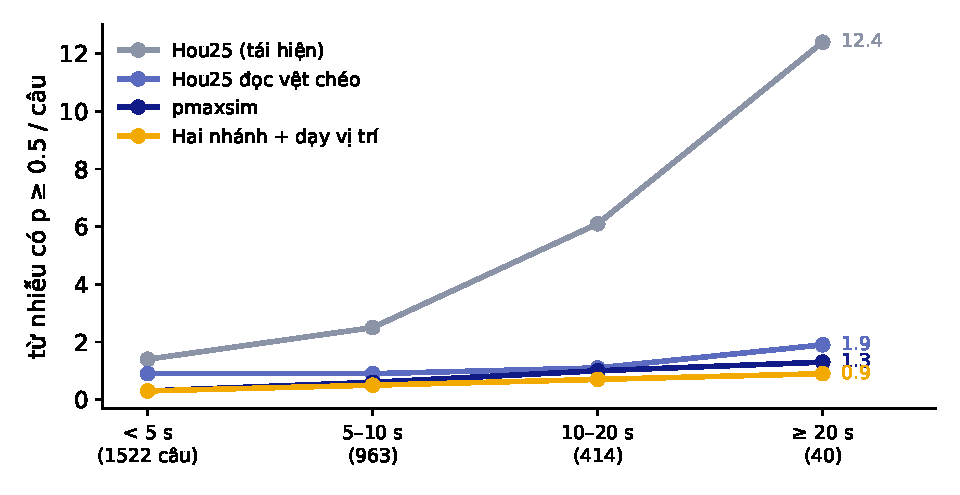
\includegraphics[width=\linewidth,height=3.9cm,keepaspectratio]{imgs/bao_nham.pdf}
\column{0.40\textwidth}
\renewcommand{\arraystretch}{1.15}\footnotesize\setlength{\tabcolsep}{4pt}
\begin{tabular}{lc}
\toprule
Câu $\geq$ 20 s & nhiễu/câu \\
\midrule
Hou25 & \bad{12.4} \\
Hou25 vệt chéo & 1.9 \\
khớp tự do & 1.3 \\
\rowcolor{Accent!15}\textbf{đề xuất} & \good{0.9} \\
\bottomrule
\end{tabular}
\par\vspace{0.15cm}
{\scriptsize\color{RiskRed}\textbf{Chưa tách được:} ``khớp tự do'' không đòi thứ tự mà vẫn thấp, nhưng nó khác Hou25 hai chỗ cùng lúc (âm vị; max thay trung bình).\par}
\end{columns}
\src{test-other N2000, từ nhiễu $p \geq 0.5$; câu $\geq$ 20 s chỉ có 40 câu. Hou25 ở đây là bản 72.6 (bản train cùng lượt ở trang 12: 6.1).}
\end{frame}

\begin{frame}{Scorer 13. Lọc list: 2000 từ \ra{} 1.9 từ/câu}
\insight{Vào 2000 từ, ra trung bình \nb{1.92 từ/câu} = \nb{1.65 đúng + 0.27 nhiễu}. Câu thật có 1.79 từ hiếm \ra{} list sau lọc \nb{gần bằng} danh sách thật. Hou25: 1.30 đúng + 1.06 nhiễu.}
\begin{columns}[T]
\column{0.42\textwidth}
{\scriptsize\textbf{Cách lọc}, mỗi câu:\par
1.\ Chấm 2000 từ, lấy top-50.\par
2.\ Hai từ \textbf{trùng chỗ} (chồng nhau $>$ 30\%) \ra{} giữ từ $p$ cao hơn. Vd.\ \texttt{pileser} (.8) và \texttt{pillar} (.4) cùng ở giây 3.0--3.6 \ra{} \bad{loại} \texttt{pillar}.\par
3.\ Giữ từ có $p \geq 0.5$.\par\vspace{0.08cm}
\textbf{Tính 1.92} (đề xuất; 2939 câu, 5248 lượt từ hiếm):\par
đúng còn = 92.4\% $\times$ 5248 = 4849 (1.65/câu)\par
nhiễu còn = 0.27 $\times$ 2939 = 794\par
tổng = 5643 / 2939 = \textbf{1.92 từ/câu}\par
precision = 4849 / 5643 = \textbf{85.9\%}\par}
\column{0.56\textwidth}
\renewcommand{\arraystretch}{1.05}\scriptsize\setlength{\tabcolsep}{3pt}
\begin{tabular}{lcccc}
\toprule
$p \geq 0.5$ & giữ đúng & nhiễu/câu & từ/câu & precision \\
\midrule
Hou25 & 73.0\% & 1.06 & 2.36 & \bad{55.2\%} \\
Hou25 vệt chéo & 88.3\% & 0.59 & 2.17 & 72.9\% \\
\rowcolor{Accent!15}\textbf{đề xuất} & \textbf{92.4\%} & \textbf{0.27} & \textbf{1.92} & \good{85.9\%} \\
\bottomrule
\end{tabular}
\par\vspace{0.06cm}
{\scriptsize\textbullet\ \textbf{Giữ đúng} = đúng còn / 5248. \textbf{Nhiễu/câu} = nhiễu còn / 2939. \textbf{Từ/câu} = tổng còn / 2939.\par
\textbullet\ Bước 2 làm Hou25 \textbf{mất} 14 điểm từ đúng (87.0 \ra{} 73.0): vị trí của nó sai (44\% tâm trúng), nên từ đúng bị coi là ``trùng chỗ'' với một nhiễu điểm cao hơn và bị loại nhầm.\par
\textbullet\ Bỏ bước 2, hạ ngưỡng 0.3 để giữ $\sim$91\% từ đúng \ra{} Hou25 precision chỉ \bad{21\%}.\par}
\end{columns}
\src{scorer/analysis/nms\_fair\_other.md (tính lại 17/11). Từ/câu tính từ hai cột trước, vd.\ Hou25: 0.730$\times$5248/2939 + 1.06 = 2.36.}
\end{frame}

\begin{frame}{Scorer 14. Chỗ yếu: từ nhiễu nghe như một từ thường}
\insight{Từ nhiễu nghe giống \nb{một từ thường} trong câu thì \nb{không có từ hiếm nào tranh chỗ} nên nó lọt \ra{} cần thêm lựa chọn ``\nb{chỗ này không có từ nào}''.}
\centering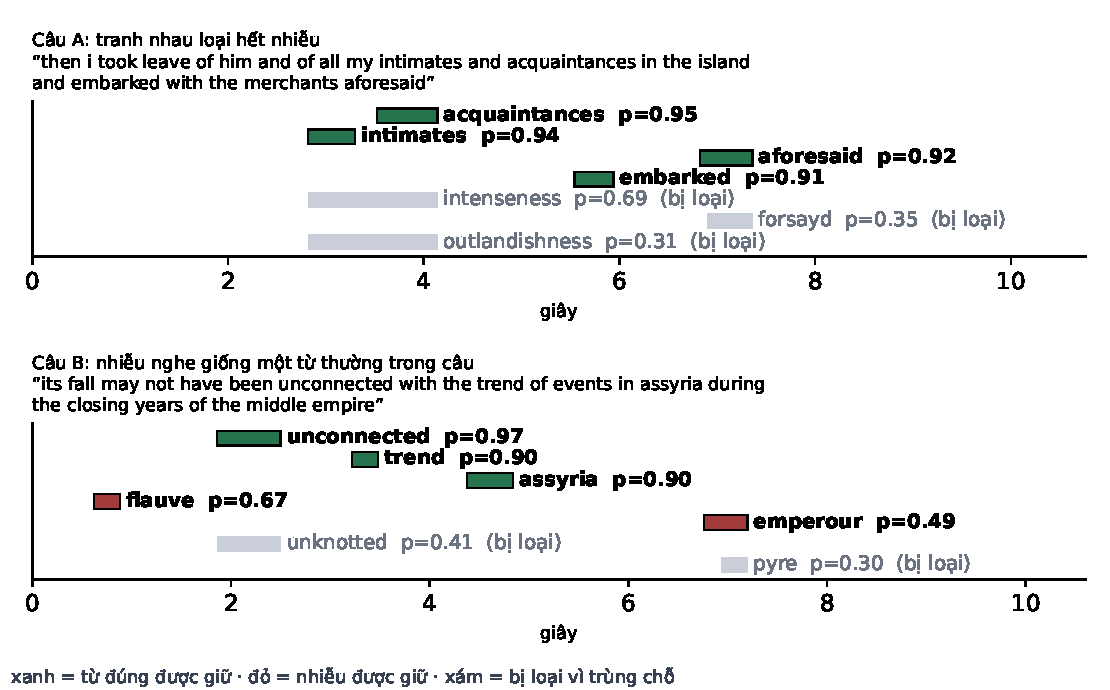
\includegraphics[width=0.92\linewidth,height=4.6cm,keepaspectratio]{imgs/tranh_nhau.pdf}\par
\raggedright{\footnotesize \textbf{Câu A:} nhiễu trùng chỗ đều \good{bị loại}. \quad \textbf{Câu B:} \texttt{flauve} $\approx$ ``fall'', \texttt{emperour} $\approx$ ``empire'' \ra{} \bad{lọt}.\par}
\end{frame}

% ==================================================================
\section{Whisper}
\begin{frame}{Whisper 1. Cách nhắc đúng lúc}
\insight{Whisper hầu như \nb{không viết từ vào sai chỗ}, nhưng hay \nb{viết thêm khi không cần}. Vị trí dùng để biết \nb{lúc nào phải im lặng}.}
\begin{columns}[T]
\column{0.52\textwidth}
{\footnotesize\textbf{Cách nhắc}, mỗi lần Whisper viết một chữ:\par\vspace{0.08cm}
1.\ Đọc alignment heads \ra{} biết Whisper đang nghe giây nào.\par\vspace{0.05cm}
2.\ Từ nào được scorer đặt ở giây đó \ra{} cộng $\lambda = 5$ vào token đầu của từ.\par\vspace{0.05cm}
3.\ Mỗi từ chỉ nhắc đến khi đã được viết ra (chặn lặp).\par}
\column{0.46\textwidth}
\renewcommand{\arraystretch}{1.15}\footnotesize\setlength{\tabcolsep}{4pt}
\begin{tabular}{lc}
\toprule
Kiểm trước (CPU) & tỉ lệ \\
\midrule
viết từ hiếm vào chỗ từ khác & \good{$\leq$ 0.36\%} \\
nhắc mọi lúc: viết thêm & \bad{24\%} \\
nhắc đúng lúc (vị trí MFA) & $\approx$ 0 \\
\bottomrule
\end{tabular}
\end{columns}
\src{Lấy giây đang nghe: Simul-Whisper (arXiv 2406.10052 §2.1). Tham số chọn trên dev-other 400 câu. SMALL\_R N6.}
\end{frame}

\begin{frame}{Whisper 2. Thắng Hou25 ở từ hiếm, không cần prompt}
\insight{B-WER (lỗi trên từ hiếm) test-other \nb{9.69 \ra{} 7.65}, test-clean \nb{5.15 \ra{} 3.83}, không cần prompt. \nb{WER tổng chưa thắng có ý nghĩa.}}
\begin{columns}[T]
\column{0.58\textwidth}
\renewcommand{\arraystretch}{1.15}\footnotesize\setlength{\tabcolsep}{4pt}
\begin{tabular}{lcc}
\toprule
WER / B-WER & test-other & test-clean \\
\midrule
không có list & 4.25 / 17.92 & 2.16 / 8.64 \\
Hou25: prompt top-50 & 3.39 / 9.69 & 1.66 / 5.15 \\
\rowcolor{Accent!15}\textbf{đề xuất + nhắc đúng lúc} & \textbf{3.22 / 7.65} & \textbf{1.58 / 3.83} \\
trần (từ + vị trí thật) & 2.99 / 5.99 & 1.53 / 2.77 \\
\bottomrule
\end{tabular}
\par\vspace{0.1cm}
{\scriptsize B-WER: lỗi chỉ tính trên các từ hiếm của câu đúng, chấm bằng script IS21 chính thức. Cùng Whisper, cùng list; ngưỡng, độ mạnh nhắc chọn trên dev-other.\par}
\column{0.40\textwidth}
{\footnotesize\textbf{So với Hou25} (khoảng tin cậy 95\%):\par\vspace{0.05cm}
B-WER other \good{$-$2.04} [$-$2.76; $-$1.37]\par
B-WER clean \good{$-$1.32} [$-$1.83; $-$0.81]\par\vspace{0.1cm}
WER other $-$0.17 [$-$0.39; +0.12] \ra{} \bad{chưa có ý nghĩa}.\par\vspace{0.15cm}}
{\scriptsize\color{RiskRed}\textbf{Chưa tách được:} lợi do scorer hay do cách nhắc. Hai bên khác cả hai thứ; thiếu dòng ``Hou25 vệt chéo + nhắc đúng lúc''.\par}
\end{columns}
\src{N2000; REPORT-1115 mục 7c (bản một model). Bản cộng điểm 2 model: 3.14 / 7.53. Thêm prompt: B-WER 6.42 nhưng lỗi ở từ thường tăng.}
\end{frame}

\begin{frame}{Whisper 3. Ba điều rút ra phía ASR}
\insight{Scorer chỉ có lời khi đưa ra \nb{(từ, $p$, vị trí)} và được dùng \nb{lúc decode}. Xếp hạng tốt hơn mà đưa vào prompt thì vô ích.}
\begin{columns}[T]
\column{0.32\textwidth}
\nbox{\textbf{1. Cần vị trí} (D2)\\[2pt]
Cùng list, nhắc mọi lúc WER 3.66, nhắc đúng lúc \good{3.22}.\\
$-$0.44 [$-$0.55; $-$0.35].}
\column{0.32\textwidth}
\nbox{\textbf{2. Prompt đã đầy}\\[2pt]
Scorer hơn Hou25 \textbf{17 điểm} Recall@1, đưa top-50 vào prompt vẫn \bad{không hơn} (10.03 so với 9.69).}
\column{0.32\textwidth}
\nbox{\textbf{3. Còn 1.7 tới trần}\\[2pt]
7.65 so với trần 5.99: \textbf{một nửa do vị trí}, một nửa do list.}
\end{columns}
\src{test-other N2000 (REPORT-1115 mục 7, 7b). Tách tới trần đo trên dev-other.}
\end{frame}

\begin{frame}{Whisper 4. List dài hơn 20 lần, B-WER chỉ tăng 0.5}
\insight{N100 \ra{} N2000: nhiễu lọt qua scorer \nb{0.04 \ra{} 0.73 từ/câu}, nhưng B-WER chỉ \nb{7.14 \ra{} 7.65}, WER \nb{2.96 \ra{} 3.22}. Từ nhiễu \nb{chỉ được nhắc ở đoạn của nó}.}
\begin{columns}[T]
\column{0.58\textwidth}
\renewcommand{\arraystretch}{1.05}\scriptsize\setlength{\tabcolsep}{3pt}
\begin{tabular}{lccccc}
\toprule
List & Recall@1 & nhiễu/câu & precision & WER & B-WER \\
\midrule
N100 & 98.2 & 0.04 & 97.8\% & 2.96 & 7.14 \\
N500 & 94.1 & 0.21 & 89.2\% & 3.04 & 7.37 \\
N1000 & 92.6 & 0.39 & 81.4\% & 3.08 & 7.47 \\
N2000 & 89.0 & 0.73 & 69.9\% & 3.22 & 7.65 \\
\midrule
\textcolor{TextGray}{không list} & -- & -- & -- & \textcolor{TextGray}{4.25} & \textcolor{TextGray}{17.92} \\
\bottomrule
\end{tabular}
\par\vspace{0.06cm}
{\tiny N$x$ = từ hiếm đúng + $x$ từ nhiễu. Ngưỡng ở đây $p \geq 0.3$ (chọn trên dev cho Whisper) nên precision N2000 là 70\%, thấp hơn 86\% ở trang 26 (ngưỡng 0.5). Giữ từ đúng 95--96\% ở mọi N.\par}
\column{0.40\textwidth}
{\scriptsize\textbf{Đọc số:}\par
\textbullet\ Mỗi câu thêm 0.7 từ nhiễu được nhắc, mà B-WER +0.51, WER +0.26 \ra{} phần lớn nhiễu được nhắc nhưng \textbf{Whisper không viết ra}: audio không ủng hộ.\par
\textbullet\ N2000: B-WER vẫn giảm \textbf{57\%} so với không list, (17.92 $-$ 7.65)/17.92.\par
\textbullet\ Phần mất khi list dài có thể do \textbf{sót từ đúng} (Recall@1 98.2 \ra{} 89.0) hơn là do viết thêm nhiễu (diễn giải, chưa tách).\par\vspace{0.06cm}}
{\tiny\color{RiskRed}\textbf{Chưa có:} Hou25 ở N100--1000 trong cùng pipeline \ra{} chưa nói được ``bền hơn Hou25''.\par}
\end{columns}
\src{test-other; scorer đề xuất (một model); tranh nhau tại chỗ; nhắc đúng lúc, không prompt. REPORT-1115 mục 7c (Recall@1 bản lọc lại: 89.0).}
\end{frame}

% ==================================================================
\section{Đúc kết}
\begin{frame}{Đúc kết}
\insight{Biết \nb{từ nằm ở đâu} làm scorer \nb{chọn đúng} và Whisper \nb{viết đúng}. Hou25 bỏ mất nó ở bước trung bình; scorer âm vị giữ nó bằng đường đi đúng thứ tự.}
\begin{columns}[T]
\column{0.32\textwidth}
\nbox{\textbf{1. Vì sao Hou25 thua}\\[2pt]\scriptsize
Trung bình mọi ô \ra{} không biết thứ tự \ra{} nhiễu rải rác thắng; câu dài càng nặng (1.4 \ra{} 12.4 nhiễu/câu).\\[1pt]
Chỉ đổi sang vệt chéo: \textbf{73.3 \ra{} 82.9}.}
\column{0.32\textwidth}
\nbox{\textbf{2. Scorer đề xuất}\\[2pt]\scriptsize
Bảng âm vị $\times$ khung, đọc hai nhánh: tự do (không sót) + thứ tự (không nhầm, ra vị trí); dạy vị trí lúc train.\\[1pt]
Recall@1 \textbf{89.3} (Hou25 72.6); tâm lệch \textbf{0.02 s}; 2000 \ra{} \textbf{1.9 từ/câu}, precision 86\%.}
\column{0.32\textwidth}
\nbox{\textbf{3. Whisper dùng vị trí}\\[2pt]\scriptsize
Nhắc đúng lúc thay prompt: B-WER \textbf{9.69 \ra{} 7.65} [$-$2.76; $-$1.37].\\[1pt]
Có vị trí so với không: WER $-$0.44.\\[1pt]
N100 \ra{} N2000: B-WER chỉ +0.5.}
\end{columns}
\vspace{0.02cm}
\yeu{\scriptsize\textbf{Chưa chắc:} WER tổng mới ngang Hou25 ($-$0.17 [$-$0.39; +0.12]); list toàn nhiễu làm WER tệ đi (4.25 \ra{} 4.51); Hou25 mới 2 epoch; mới có Whisper.}
\src{test-other, N2000 trừ khi ghi khác.}
\end{frame}

\end{document}
